\documentclass[review]{elsarticle}

\usepackage{lineno,hyperref}
\usepackage{color}
\usepackage{xcolor}
\usepackage{amssymb,amsmath}
\usepackage{graphicx}
\usepackage{blindtext}
\usepackage{multirow}
\usepackage{algorithmic}
\usepackage{algorithm}
\usepackage{enumerate}
%\usepackage{subcaption,graphicx}
\usepackage{subfig}
\modulolinenumbers[5]

\begin{document}

\begin{frontmatter}

\title{A Novel Adaptive Approximate Bayesian Computation Method for Inverse Heat Conduction Problem}

\author[mymainaddress,mysecondaryaddress]{Yang Zeng}

\author[mymainaddress,mysecondaryaddress]{Shuai Zhang}

\author[mymainaddress,mysecondaryaddress]{Yong Cai}

\author[mysecondaryaddress]{Hu Wang\corref{mycorrespondingauthor}}
\cortext[mycorrespondingauthor]{Corresponding author}
\ead{wanghu@hnu.edu.cn}

\address[mymainaddress]{College of Mechanical and Vehicle engineering, Hunan University}
\address[mysecondaryaddress]{State Key Laboratory of Advanced Design and Manufacturing for Vehicle Body}

\begin{abstract}
Bayesian approach has been widely used in inverse heat conduction problem (IHCP). However, due to either computationally prohibitive or analytically unavailable, its likelihood function is always intractable. In this study, to circumvent the intractable likelihood function, an approximate Bayesian computation (ABC) is extended to IHCP. Howerver, in the ABC, massive expensive forward simulations are needed. It might lead to prohibited computational cost. In order to improve the efficiency of the ABC-IHCP, two strategies are proposed in this study. At first, in order to improve the convergence rate of ABC and reduce the number of samples, a none-parametric population Monte Carlo (NPMC) is proposed to determine the decreasing tolerance value adaptively. Secondly, in order to save the expensive computational cost of heat conduction simulation, the fast computational techniques are utilized. Based on the characteristics of the linear and nonlinear heat transfer problems, two heat conduction solvers are developed, respectively. The linear solver is based on superposition principle. As for the nonlinear problem, the fast and accurate reanalysis solver is suggested. Finally, the accuracy and efficiency of the suggested methods are verified with two numerical examples.
\end{abstract}

\begin{keyword}
Inverse Heat Conduction Problem (IHCP), Approximate Bayesian Computation (ABC), Reanalysis, Non-parametric Population Monte Carlo (NPMC)
\end{keyword}

\end{frontmatter}

\section{Introduction}

The purpose of the inverse heat conduction problem (IHCP) is to estimate unknowns of the heat conduction given the observations. Since these estimations are generally not unique or unstable due to small perturbation of the observations \cite{murio2011mollification, wang2004bayesian}, the IHCP is often ill-posed. In order to obtain more reliable estimations, many deterministic methods have been developed such as Tikhonov regularization \cite{tikhonov2013numerical,bozzoli2014estimation,okamoto2007regularization, yang2010method, alifanov2012inverse, woodbury2013estimation}, iterative regularization\cite{alifanov2012inverse}, sequential function specification method (SFM) \cite{alifanov2012inverse, cabeza2005sequential, chantasiriwan2001algorithm}, Levenberg-Marquardt (LM) method \cite{rouquette2007estimation} and the Fourier regularization method \cite{mierzwiczak2010application, dou2009optimal} and so on. In addition, the filtering technique approach\cite{bozzoli2013experimental, bozzoli2011comparative} is a very well alternative deterministic methods. Besides, some stochastic methods have been also widely concerned \cite{wang2004bayesian,wang2005using, liu2008bayesian, parthasarathy2008estimation, massard2012estimation}. \textcolor{red}{Parthasarathy \cite{parthasarathy2008estimation} pointed out that the stochastic methods were data driven and could achieve a very good performance to the ill-posed problem.}  Among these stochastic methods, one of the most general and versatile method is Bayesian method \cite{wang2004bayesian,wang2005using, liu2008bayesian, parthasarathy2008estimation}. In Bayesian framework, the ill-posed inverse problem can be regularized with the prior distribution modelling. Then robust posterior functions can be achieved. 

However, in the practical problems, the likelihood function of Bayesian is always intractable due to either computationally prohibitive or analytically unavailable. To circumvent this intractable likelihood function, an approximate Bayesian computation (ABC) was proposed by Pritchard \cite{pritchard1999population} with a rejection technique as shown in Fig.\ref{fig:ABC}. \textcolor{red}{In order to improve the efficiency or make it more flexible, researchers have developed a series of ABC forms.} The simplest ABC form is based on rejection sampling algorithm \cite{beaumont2002approximate, bortot2007inference}. However, this method suffers a rather low acceptance rate if the prior is quite different from the posterior. To improve the efficiency, Markov chain Monte Carlo (MCMC) method\cite{marjoram2003markov} was extended to ABC. However, in the ABC-MCMC, the acceptance rate depends on the proposal mechanism and poor proposal mechanism would lead to a very low acceptance rate \cite{beaumont2009adaptive}. To avoid the pool proposal mechanism, particle filtering was extended to the ABC. The ABC particle filtering can be classified as three forms: Partial rejection control (PRC) \cite{sisson2007sequential}, population Monte Carlo (PMC) \cite{beaumont2009adaptive,beaumont2010approximate} and sequential Monte Carlo (SMC) \cite{toni2009approximate}. For ABC-PRC, it might lead to biased estimation of posteriors \cite{beaumont2009adaptive}. The ABC-PMC and ABC-SMC are similar except that the kernel of ABC-PMC is Gaussian and adaptive. Several researchers focus on adaptive SMC in ABC such as partial rejection mechanism \cite{del2012adaptive} and adaptive SMC \cite{lenormand2013adaptive}. It should be noted that ABC-PMC is still the versatile method in practice.

According to existed literatures, it seems that the ABC has not been applied to heat conduction yet. In this study, we hope the ABC can avoid the intractable likelihood function of heat conduction problem and obtain stable unknown boundary condition with given temperature field. In the traditional ABC-PMC, given the summary static, the convergent rate of ABC only depends on the tolerance value. If the tolerance value is not suitable, the efficiency might be quite low. In this study, in order to improve the convergent rate of ABC and reduce the number of samples, a none-parametric population Monte Carlo (NPMC) is proposed to determine the decreasing tolerance value adaptively. In the suggested method, the convergent rate is controllable. Compared with traditional ABC-PMC method, predefining tolerance values are not needed and the efficiency can be improved significantly.

\begin{figure}
    \centering
    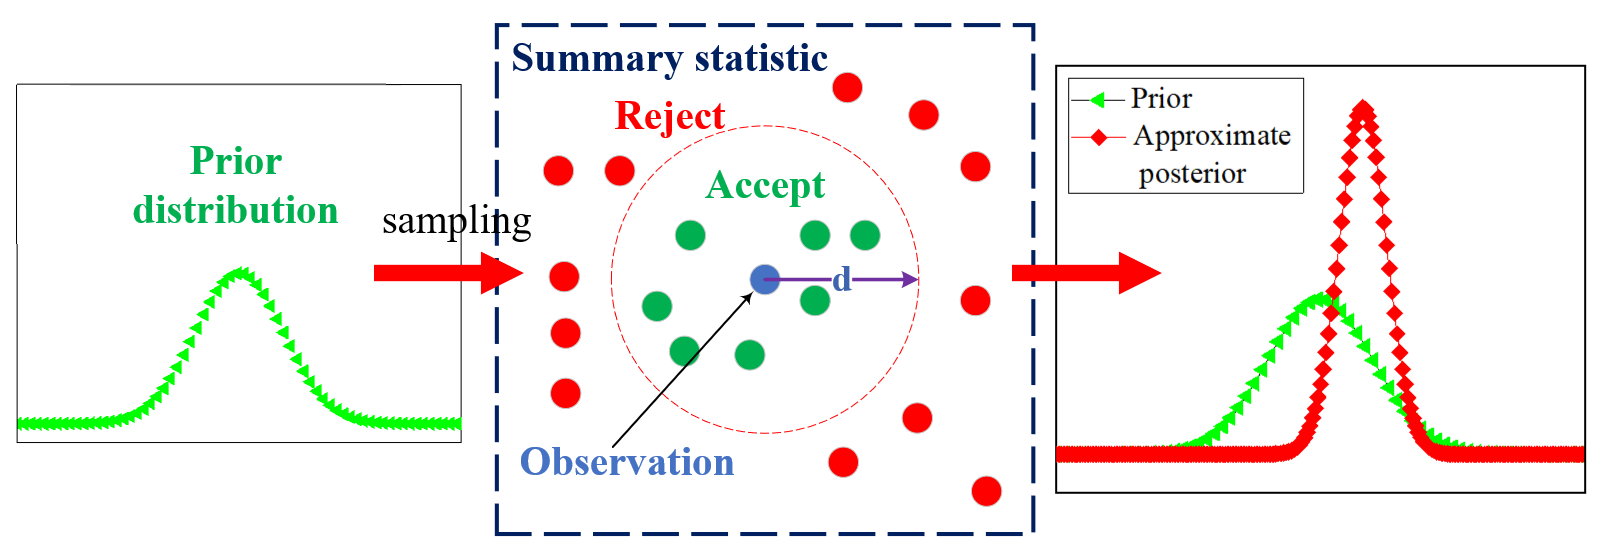
\includegraphics[width=0.95\textwidth]{fig/ABC.png}
    \caption{The framework of ABC}
    \label{fig:ABC}
\end{figure}
 
In addition, in order to obtain accurate approximate posteriors, massive forward simulations are needed. Theoretically, several kinds of methods can be used to evaluate heat conduction problem such as finite difference method (FDM)  \cite{alifanov2012inverse, yang1998solving, yang1999determination}, finite element method (FEM) \cite{alifanov2012inverse,krizek1998finite, palma2012non}, boundary element method (BEM) \cite{sutradhar2004simple, tanaka2006dual, martin1996inverse}, meshless method \cite{yan2009meshless} and Edge-smooth FEM (ES-FEM)\cite{cui2016steady, nguyen2011adaptive}. Among these methods, FEM is still a very stable and widely used method\cite{fatullayev2002numerical}. However, the computational cost based on FEM is always expensive, especially for the dynamic IHCP. In order to reduce the computational cost of simulation, the fast and accurate computational techniques are developed instead of the FE simulations. In this study, due to the character of IHCPs\cite{bozzoli2014estimation}  the superposition is used for linear problem and the combined approximation (CA) reanalysis is used for nonlinear problem. Reanalysis is based on the FEM framework. However, the reanalysis \cite{wang2016seen, wang2013parallel, wang2017reanalysis} focuses on the modification of the modified system equations. Generally, a far less dimensional system of linear equations is solved in reanalysis compared with the standard FEM and the efficiency of evaluation can be significantly improved. The CA method is one of the most versatile and widely used approximate reanalysis method. It was originally proposed by Kirsch and Moses \cite{krizek1998finite, kirsch2001exact}. He demonstrated that the CA reanalysis can achieve accurate approximations of displacements, stresses and forces. 

In addition, sensitive analysis is significant in inverse problem \cite{chantasiriwan2001algorithm} since it can figure out the influence on response from the perturbation of parameters. The sensitive analysis can filter the parameters which have little influence on response. In this study, before inverse problem, the Random Sampling-High Dimensional Model Representation (RS-HDMR) \cite{li2002practical,wang2017global} is used to analysis the sensitive of unknown parameters and filter the insensitive parameters. The accuracy and efficiency of the proposed methods are tested with two numerical examples.

The remainder of the paper is organized in the following manner: Sec.2 gives the basic architecture of forward heat conduction solvers. In Sec.3, the Bayesian formula and ABC are introduced. Then the suggested adaptive NPMC method is presented in Sec.4. In Sec.5, the suggested methods are verified by numerical examples. Conclusion are summarized in Sec.6.


\section{Forward heat conduction solvers}
\subsection{Basic formula}
The governing equation of forward heat conduction problem can be given as
\begin{equation}
    \nabla \cdot (k(T)\nabla T) + Q  = \rho c(T) \frac{T}{t}
    \label{eq:govening equation}
\end{equation}

\noindent where $T$ represents the temperature field, $Q$, $\rho$ and $c$ are the heat generation, the material density and the specific heat, respectively, $k$ is the thermal conductivity. $t$ is time. In this differential problem, the boundary conditions are:
\begin{itemize}
    \item Dirichlet boundary condition: $T|_{\Gamma} = T_k$
    \item Neumann boundary condition: $-k \frac{\partial T}{\partial \mathbf{n}}|_{\Gamma}=q_0$
    \item Robin boundary condition: $-k \frac{\partial T}{\partial \mathbf{n}}|_\Gamma=h_c (T-T_{\infty})$
    \item Adiabatic boundary condition: $-k \frac{\partial T}{\partial \mathbf{n}}|_\Gamma=0$
\end{itemize}
\noindent where $T_k$ and $T_\infty$ are given temperature and environmental temperature, respectively and $q_0$, $h_c$ and $\mathbf{n}$ represent the heat flux, the convection coefficient and the unit outward normal to the boundary, respectively. FE method is used to solve Eq.\ref{eq:govening equation}. \textcolor{red}{The discrete form of Eq.\ref{eq:govening equation} can be given as}

\begin{equation}
    \mathbf{K} \mathbf{T}+\mathbf{N}\frac{\partial \mathbf{T}}{\partial t} = \mathbf{Q}
    \label{eq:FEM}
\end{equation}

\noindent where
\begin{equation*}
    \mathbf{K} =  \mathbf{K}_T+\mathbf{K}_T^h 
\end{equation*}

\begin{equation*}
    \mathbf{K}_T = \int_\Omega \mathbf{B}^T \mathbf{k} \mathbf{B} d \Omega
\end{equation*}

%\begin{bmatrix} k_x & 0 & 0\\ 0 & k_y & 0\\ 0 & 0 & k_z\end{bmatrix}

\begin{equation*}
    \mathbf{K}_T^h = \int_\Gamma h_c \mathbf{H}^T \mathbf{H} d \Gamma
\end{equation*}


\noindent \textcolor{red}{where $\mathbf{H}$ is the shape function matrix, and $\mathbf{B}$ is its derivative, $\mathbf{k}$ is the thermal conductivity matrix.} The $\mathbf{N}$ is the thermal capacitance matrix and given as:

\begin{equation*}
    \mathbf{N} = \int_\Omega \rho c\mathbf{H}^T\mathbf{H} d \Omega
\end{equation*}

\textcolor{red}{The $\mathbf{Q}$ consists of several boundary conditions:}

\begin{equation*}
    \mathbf{Q} = \mathbf{Q}_q+\mathbf{Q}_c
\end{equation*}

\begin{equation*}
    \mathbf{Q}_q = \int_\Gamma -q \mathbf{H}^T d\Gamma
\end{equation*}

\begin{equation*}
    \mathbf{Q}_c = \int_\Gamma \mathbf{H} h_c (T_\infty-T)d \Gamma
\end{equation*}

\subsection{\textcolor{red}{Linear heat conduction solver}}
In this study, the backward difference technique is used to avoid oscillation \cite{feng2016fast}. $\frac{\partial \mathbf{T}(t)}{\partial t}$ can be written as 

\begin{equation}
    \frac{\partial \mathbf{T}(t)}{\partial t} = \frac{\Delta \mathbf{T}(t)}{\Delta t} + O(\Delta t) = \frac{\mathbf{T}(t)-\mathbf{T}(t-\Delta t)}{\Delta t} + O(\Delta t) 
    \label{eq:BD}
\end{equation}

Substitute it into Eq.\ref{eq:FEM}, it has:

\begin{equation}
    (\mathbf{K} + \frac{\mathbf{N}}{\Delta t})\Delta \mathbf{T}(t) = \frac{\mathbf{Q}-\mathbf{K}\mathbf{T}(t-\Delta t)}{\Delta t}
    \label{eq:BD-FEM}
\end{equation}

\textcolor{red}{When Robin boundary condition is not considered (not apply or ignore from sensitive analysis) and the  $k$ is a constant, the forward problem will be linear for both static and dynamic heat conduction problem. Thus, $\left(\mathbf{K}+\frac{\mathbf{N}}{\Delta t}\right)$ is fixed for different boundary conditions. Therefore the inverse of it can be determined before. For the static issue, the forward problem can be solved by:}

\begin{equation}
    \mathbf{T} = \mathbf{K}^{-1}\mathbf{Q}
    \label{eq:static-linear}
\end{equation}

\noindent \textcolor{red}{where $\mathbf{Q}$ can be any boundary condition. For dynamic issue, the forward problem can be solved by}
\begin{equation}
    \Delta \mathbf{T}(t) = \left( \mathbf{K}+\frac{\mathbf{N}}{\Delta t}\right)^{-1} \left(\frac{\mathbf{Q}-\mathbf{K}\mathbf{T}(t-\Delta t)}{\Delta t}\right)
    \label{eq:dynamic-linear}
\end{equation}

\textcolor{red}{Suppose there are $s$ boundary condition parameters, $y_i$ is its value. The Eq.\ref{eq:static-linear} can be rewritten as}

\begin{equation}
    \left\{\begin{array}{lr}
    \mathbf{v}_i = \mathbf{K}^{-1}\mathbf{q}_i\\
    \mathbf{T} = \sum_{i=1}^2 y_i\mathbf{v}_i
  \end{array}
\right.
\end{equation}

The Eq.\ref{eq:dynamic-linear} can be rewritten as

\begin{equation}
    \left\{\begin{array}{lr}
    \mathbf{v}_i = \left( \mathbf{K}+\frac{\mathbf{N}}{\Delta t}\right)^{-1} \frac{\mathbf{q}_i}{\Delta t}\\
    \mathbf{K}' = \left( \mathbf{K}+\frac{\mathbf{N}}{\Delta t}\right)^{-1}\mathbf{K}\\
    \Delta\mathbf{T} = \sum_{i=1}^s y_i*\mathbf{v}_i-\mathbf{K}'\frac{\mathbf{T}(t-\Delta t)}{\Delta t}
  \end{array}
\right.
\end{equation}

\noindent \textcolor{red}{where $\mathbf{q}_i$ is $i_{th}$ boundary condition caused by unit value.}

\subsection{\textcolor{red}{Noninear heat conduction solver}}
\textcolor{red}{For the static issue, if $h_c$ of Robin boundary condition is needed to be determined, the $\mathbf{K}$ will vary in each forward problem. It leads to nonlinear static issue. Thus the varying forward problem can be written as}

\begin{equation}
    \left\{\begin{array}{lr}
    \mathbf{K}_0 \mathbf{T}  =  \mathbf{Q}_0\\
    (\mathbf{K}_0+\Delta \mathbf{K}) \mathbf{T}  =  \mathbf{Q}_0+\Delta \mathbf{Q}
  \end{array}
\right.
\end{equation}

\noindent \textcolor{red}{where the $\mathbf{K}_0$ and $\mathbf{Q}_0$ are the parameters of first forward problem and $\Delta \mathbf{K}$ is caused by varying $h_c$ of Robin boundary condition and $\Delta \mathbf{Q}$ is caused by all boundary conditions in the following forward problems.}

\textcolor{red}{As for dynamic issue, $k$ may depend on the current temperature. In addition, Robin boundary condition may vary with time. This leads to a nonlinear dynamic issue. The first step of Eq.\ref{eq:BD-FEM} is given as}
\begin{equation}
    \mathbf{K}_0 \Delta \mathbf{T} = \mathbf{R}_0
\end{equation}
\noindent where 
\begin{equation*}
    \mathbf{K}_0 = \mathbf{K}+\frac{\mathbf{N}}{\Delta t}
\end{equation*}
\begin{equation*}
    \mathbf{R}_0 = \frac{\mathbf{Q}-\mathbf{K}\mathbf{T}_0}{\Delta t}
\end{equation*}

The following steps can be written as 
\begin{equation}
    \mathbf{K}_t \Delta \mathbf{T} = \mathbf{R}_t
    \label{eq:dyna-delta}
\end{equation}

\begin{equation*}
    \left\{\begin{array}{lr}
    \mathbf{K}_t &= \mathbf{K}_0+\Delta \mathbf{K}\\
    \mathbf{R}_t &= \mathbf{R}_0+\Delta \mathbf{R}
  \end{array}
\right.
\end{equation*}

\noindent \textcolor{red}{where $\Delta\mathbf{K}$ is caused by varying thermal conductivity and varying $h_c$ of Robin boundary condition and $\Delta \mathbf{R}$ is caused by varying boundary condition and varying temperature field. The CA reanalysis method is very efficient to this issue since it focuses on the modified response $\mathbf{T}_m$ without solving complete equilibrium equation}
\begin{equation}
    \mathbf{K}_t\mathbf{T}_m = \mathbf{R}_t
    \label{eq:local}
\end{equation}
In the CA method, the $\mathbf{T}_m$ is approximated by linear combination
\begin{equation}
    \mathbf{T}_m = y_1 \mathbf{r}_1+y_2 \mathbf{r}_2+,\cdots, y_s \mathbf{r}_s = \mathbf{r_B}\mathbf{y}
    \label{eq:basisvector}
\end{equation}
\begin{equation}
    s \ll n
\end{equation}

\noindent \textcolor{red}{where $\mathbf{r}_1, \mathbf{r}_2, \cdots, \mathbf{r}_s$ are the basis vectors, $s$ is the number of vectors, $\mathbf{y}$ is the coefficient which needs to be determined. The detail of basis vectors is referred in \cite{krizek1998finite, kirsch1998improved}. $n$ is the degree of original problem. Substitute Eq.\ref{eq:basisvector} to Eq.\ref{eq:local} and premultiply $\mathbf{r_B}^T$, it has}
\begin{equation}
    \mathbf{K}_R\mathbf{y}=\mathbf{R}_R
    \label{eq:reduced}
\end{equation}

\begin{equation*}
    \left\{\begin{array}{lr}
    \mathbf{K}_R = \mathbf{r_B}^T\mathbf{K}_t\mathbf{r_B}\\
    \mathbf{R}_R = \mathbf{r_B}^T\mathbf{R}_t
  \end{array}
\right.
\end{equation*}

\textcolor{red}{With Eq.\ref{eq:reduced}, the $\mathbf{y}$ can be determined. Thus, the $\mathbf{T}_m$ can be determined according to Eq.\ref{eq:basisvector}. Since $ s\ll n$, solving Eq.\ref{eq:reduced} is much more efficient than solving Eq.\ref{eq:local} or Eq.\ref{eq:dyna-delta} directly. It should be noted that the CA in static forward problem is based on the first sample while in dynamic forward problem it is based on the first iteration of each forward problem.}

\section{Approximate Bayesian Computation}
The forward problem of heat conduction is to infer $\mathbf{T}$ given all parameters and boundary conditions. Conversely, the IHCP is defined as inferred the boundary conditions given the temperature field in this study. Bayesian approach has been widely used in the IHCP. The formula is given as

\begin{equation}
    P(\theta | D) \propto P(D|\theta) \cdot P(\theta)
    \label{eq:Bayesian}
\end{equation}

\noindent \textcolor{red}{where $\theta$ is the unknowns, $P(\theta)$ is the prior PDF, $P(D|\theta)$ is the likelihood function, $D = {d_1,d_2,\dots,d_N}$ denotes observations.}

When there are numerous observations, the estimation of likelihood function in Bayesian framework may be intractable. To circumvent this intractable estimation, the ABC is proposed. The detail is as shown in Fig.\ref{fig:ABC}. Suppose that the unknowns $\theta'$ simulates from a given distribution $P(\theta)$ (usually the prior) and calculate the response of system with , the is accepted only if the simulation $Y$ is very close to measure data $D$. It should be noted that if  $Y=D$, the is the exact posterior sample. However, it is too difficult to obtain. A distance $d(Y,D)\leq \varepsilon$ is used to represent the closeness between $Y$ and $D$. $Y$ and $D$ are always high-dimensional. This could lead to a poor accepted rate. To address this problem, the measured data is always replaced by its summary statistics\cite{joyce2008approximately,fearnhead2012constructing}. The detail of the summary statistics refers to Cox \cite{cox2006principles}. Then we have

\begin{equation}
    P(\theta|D) = P(\theta|Y=D)\approx P(\theta|d(y,D)\leq \varepsilon) \approx P(\theta|d(S(Y),S(D))\leq \varepsilon)
    \label{eq:ABC}
\end{equation}

According to Ref\cite{beaumont2002approximate}, this result will be exact, if the summary statistics $S(\cdot)$ and $\varepsilon$ are chosen properly.

\section{Non-Parametric Population Monte Carlo method}

\subsection{Brief introduction of Population Monte Carlo Method}

Beaumont et al.\cite{beaumont2009adaptive} extended the ABC technique with the population Monte Carlo sampling. In this method, the decreasing sequence of tolerance level $\varepsilon_t,(1\leq t \leq T)$ is predefined. At initial step, the sample $\Theta^{(1)}$ generates from a given distribution such as prior $P(\theta)$. Then, in arbitrary step $t (t>1)$, the sample $\Theta^{(t)}$ derives from $\Theta^{(t-1)}$ via a particle filter methodology. Namely a particle $\theta_i^{(t)}$ randomly samples from $\Theta^{(t-1)}$ with weights $\left( w_i^{(t-1)}\right)_{i=1,\cdots,N}$ and the new particle $\theta_i^{(t)}$ samples from an adaptive Gaussian Markov transition kernel $q(\theta|\theta^*)$. The $\Theta^{(t)}, t=1,2,\cdots,T$ is accepted with $d(S(Y),S(D))\leq \varepsilon_t$. It should be noted that in the adaptive Gaussian kernel $q(\theta|\theta^*)$ the mean is $\theta^*$ and the variance is twice the weighted empirical variance of particle $\Theta^{(t-1)}$. The weights $\left( w_i^{(t)}\right)_{i=1,\cdots,N}$ on each particle assigned in the previous iteration is

\begin{equation}
    w_i^t \propto \frac{P(\theta_i^t)}{\sum_{j=2}^T W_j^{(t-1)q(\theta_i^t|\theta_j^{(t-1)})}}
    \label{eq:pmc-weight}
\end{equation}

In the PMC, all coefficients are adaptive except the decreasing sequence of tolerance level $\varepsilon_t,(1\leq t \leq T)$. Unfortunately, it can affect the computational cost a lot. In order to reduce the computational cost, we propose an ad hoc adaptive method to determine $\varepsilon_t,(1\leq t \leq T)$ at each iteration. The detail of this algorithm is explained with a benchmark.

\subsection{Non-Parametric Population Monte Carlo}
The description of NPMC is presented with a benchmark case. In this case, a component applied by Robin boundary condition is presented as shown in Fig.\ref{fig:benchmark_geo}. The heat conductivity coefficient is $k =1 W/(m \cdot K)$. Suppose that in both sides $h_c$ is known and equal to $20W/m^2\cdot K$. The $T_\infty$ in both sides is unknown and need to be identified given observations with ABC. The observations are the temperature field with $T_{\infty, L}=100 ^{\circ}C$ and $T_{\infty, R}=30^{\circ}C$  which are the left and right the Robin boundary condition, respectively. 

\begin{figure}
    \centering
    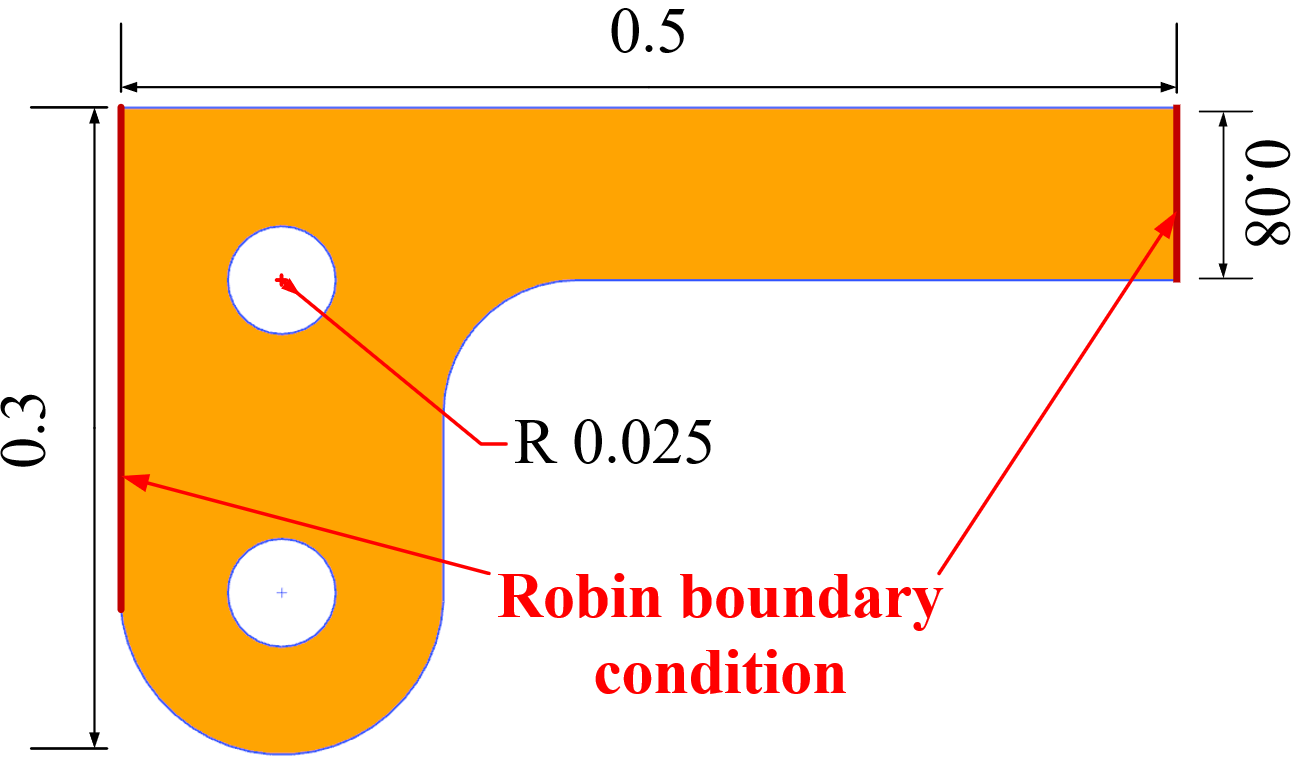
\includegraphics[width=0.7\textwidth]{fig/geo-benchmark.jpg}
    \caption{The geometry of benchmark case}
    \label{fig:benchmark_geo}
\end{figure}

As mentioned before, the tolerance value can affect the computational cost a lot. However, the connection between tolerance value and computational cost is unknown. To begin with, we need figure it out. In order to quantify this connection, we predefine a sample pool with $N_p$ samples. The samples in pool are generated based on the PMC rule without the rejected step. At the first iteration, the $N_p$ samples in pool are generated from the prior distribution. At arbitrary step $t (t>1)$, the samples in pool are generated from the particle $\Theta^{(t-1)}$. Suppose that at specified iteration, the tolerance value is $\varepsilon_t, (1\leq t \leq T)$, then $N_{acc}$ samples with $d(S(Y),S(D))<\varepsilon_t$ in pool can be accepted as part of the particle. Then the accepted rate ratio and the number of samples which is need to obtain $N$ particles at this iteration are given as

\begin{equation}
    p_{accept} = \lim_{N_p \to \infty} \frac{N_{acc}}{N_p}
\end{equation}

\begin{equation}
    N_{need} = \frac{N}{P_{accept}} = \lim_{N_p \to \infty} \frac{N\cdot N_p}{N_{acc}}
\end{equation}

For arbitrary range from 1 to $N_p$, the maximum $d$ among the accepted samples will approximately equal to current tolerance value $\varepsilon_t, (1\leq t \leq T)$. Thus the connection between computational cost and the tolerance value at specified iteration can be obtained. For example, these connections at the $1^{st}$ , $4^{th}$ , $7^{th}$  and $11^{th}$ iterations of the benchmark are presented in Fig.\ref{fig:connection}. From Fig.\ref{fig:connection}, it can be shown that when the tolerance value at specified iteration decreases, the computational cost increases slowly first and then more and more rapidly. It means when the tolerance value is chosen to be too small at the current iteration, the computational cost is expensive. For example, when the tolerance value approaches 0, the number of simulations approaches $N\cdot N_p$. If the $N_p = 2000$ as shown in Fig.\ref{fig:connection}, the number of computational samples could might be over 4,000,000. This computational cost is extremely expensive. Conversely, if the tolerance value at presented iteration is chosen to be too large, the computational cost at current iteration is low. However, in order to obtain accurate approximate posterior, more iterations are needed. Then the total computational cost could be also expensive. Thus, in order to reduce the computational cost, the tolerance value and the computational cost at each iteration should reach a balance that computational cost and tolerance value are small simultaneously. From the connection as shown in Fig.\ref{fig:connection}, the balance that minimizing computational cost and tolerance value simultaneously can be obtained by minimizing the distance from the connection curve to original point. Thus, this issue can be transformed to an optimization problem. In this study, three distances are presented to analysis this issue. They are Manhattan distance, Euclidean distance and Chebyshev distance. Then, the form of optimization is given as

\begin{figure}
    \centering
    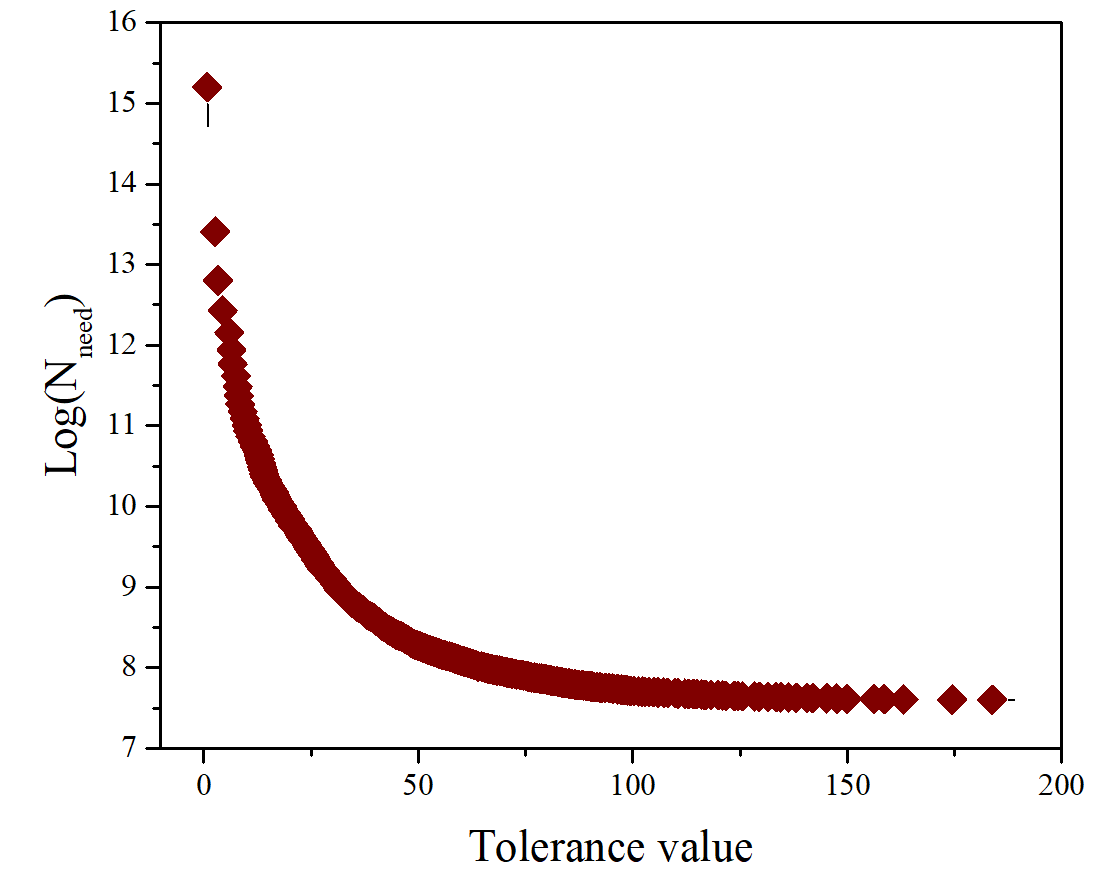
\includegraphics[width = 0.46\textwidth]{fig/connection1.png}
    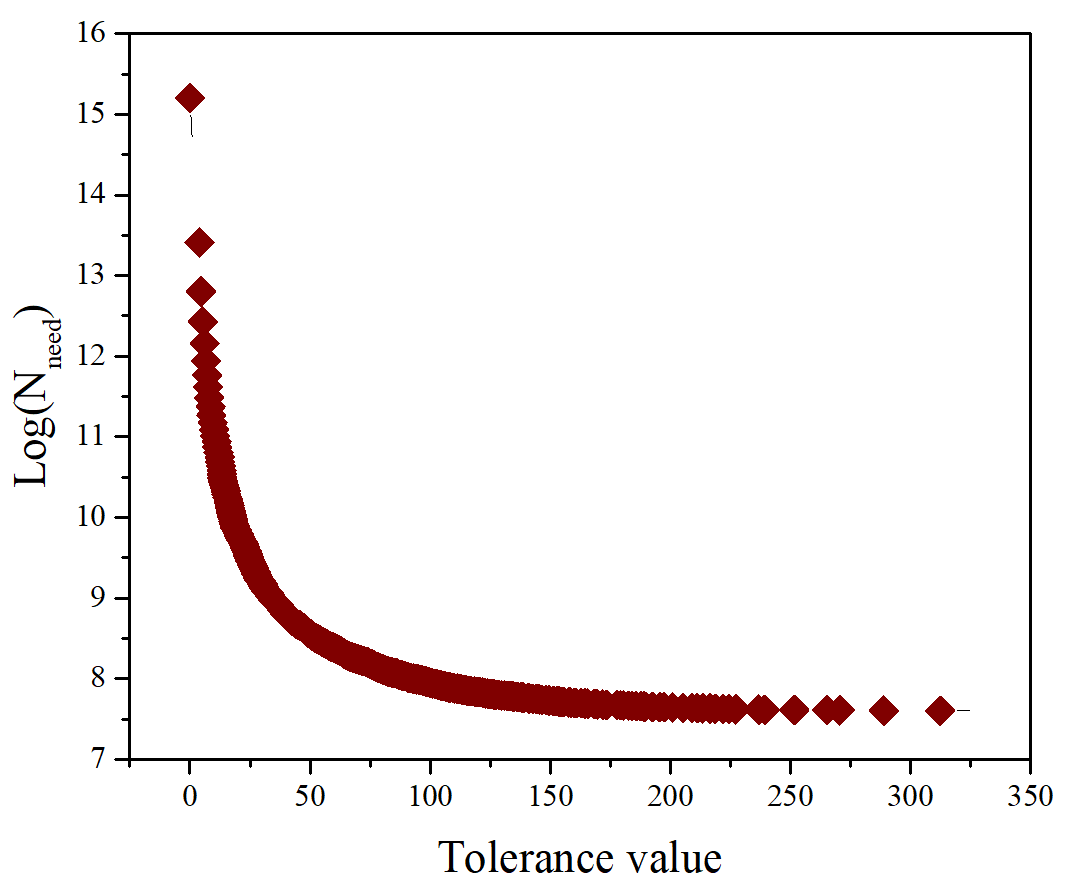
\includegraphics[width = 0.45\textwidth]{fig/connection2.png}
    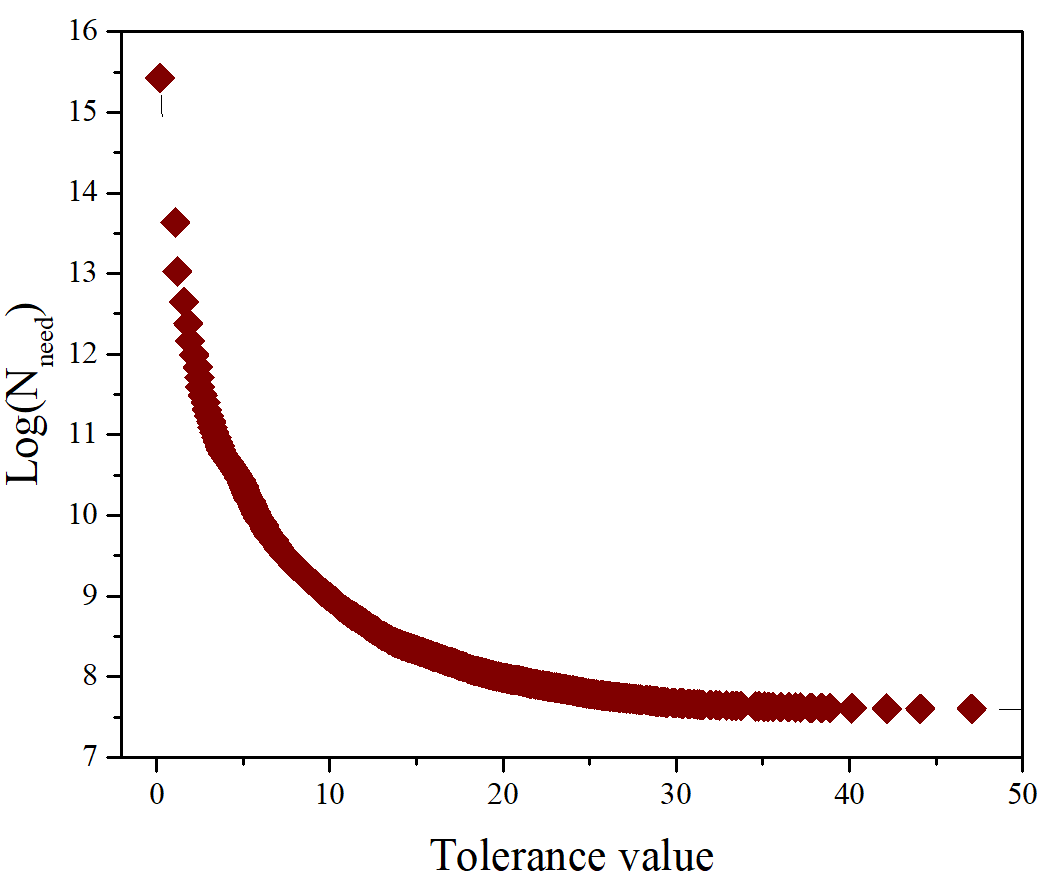
\includegraphics[width = 0.45\textwidth]{fig/connection3.png}
    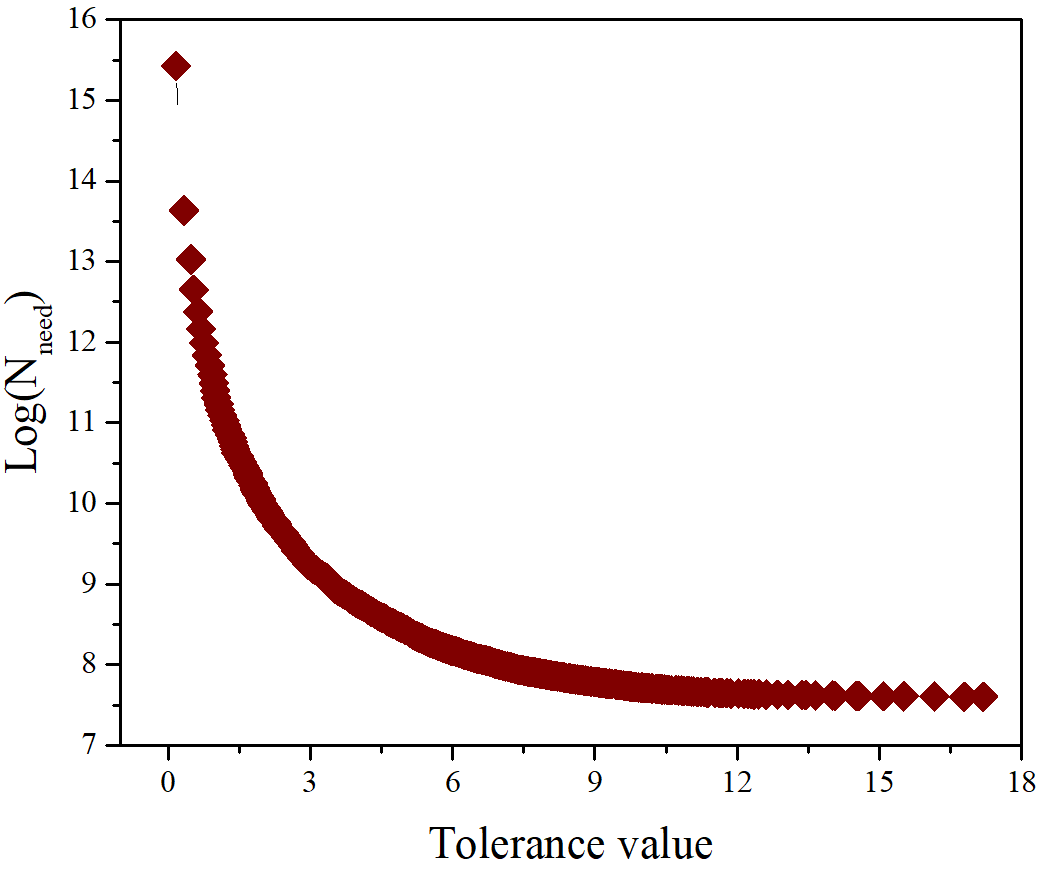
\includegraphics[width = 0.45\textwidth]{fig/connection4.png}
    \caption{The connections between computational cost and Tolerance tolerance value at 1st , 4th , 7th and 11th iterations of benchmark}
    \label{fig:connection}
\end{figure}

\begin{equation}
    \left\{\begin{array}{lr}
    min & |\log(N_{need})|+ |\varepsilon_t|\\
    s.t. & f(N_{need, \varepsilon_t})=0
  \end{array}
\right.
\label{eq:Man}
\end{equation}

\begin{equation}
    \left\{\begin{array}{lr}
    min & (\log(N_{need}))^2+ \varepsilon_t^2\\
    s.t. & f(N_{need, \varepsilon_t})=0
  \end{array}
\right.
\label{eq:Euc}
\end{equation}

\begin{equation}
    \left\{\begin{array}{lr}
    min & max(\log(N_{need}), \varepsilon_t)\\
    s.t. & f(N_{need, \varepsilon_t})=0
  \end{array}
\right.
\label{eq:che}
\end{equation}

\noindent where $f(N_{need, \varepsilon_t})=0$ is the connection between computational cost and tolerance value obtained from the sample pool. The target functions in Eq.\ref{eq:Man}-\ref{eq:che} are Manhattan distance, Euclidean distance and Chebyshev distance, respectively.

We extended this strategy to PMC with different distance functions in \cite{lenormand2013adaptive}. Since no extra parameters are needed, we call this method preliminary Non-Parametric population Monte Carlo method (PNPMC). In order to examine the efficiency of this ad hoc strategy, the APMC\cite{lenormand2013adaptive} is modified (MAPMC) to the version that only adaptive mechanism of determining remain and used to compared with PNPMC. These two algorithms are implemented for the benchmark with based on the setting in benchmark. Figure \ref{fig:bench_cost} shows the results. From Fig.\ref{fig:bench_cost}, it can be shown that the efficiency of MAPMC depends on predefined $\alpha$. When it is chosen properly (like $\alpha=0.3$), this method would be rather efficient. Conversely, if the is not proper suitable, the efficiency would might deteriorate much. Unfortunately, in for the real engineering problem, there is no useful prior information about $\alpha$. As for the PNPMC, no extra coefficient is needed. It means that this method is easier to be implemented. The computational cost of the PNPMC with Euclidean distance and Chebyshev distance PNPMC reaches quite low computation of APMC with  $\alpha=0.3$  as shown in Fig.\ref{fig:bench_cost}. It should be noted that in the benchmark the computational cost of the APMC with $\alpha=0.3$ is not the lowest but a comparatively low one. Therefore, the PNPMC is more efficient. It suggests that the proposed strategy with Euclidean distance and Chebyshev distance in PMC is more efficient. To further reduce the computational cost, we extended the PNPMC as Non-Parametric PMC (NPMC) with the idea that the samples with $d<\varepsilon_t$ in last particles can be remained in the next iteration\cite{lenormand2013adaptive}. The details of algorithm are presented in \textbf{Algorithm 2}. From Fig.\ref{fig:bench_cost}, it can be seen found that the proposed efficiency of the NPMC improves a lot compared with that of the PNPMC.

\begin{figure}
    \centering
    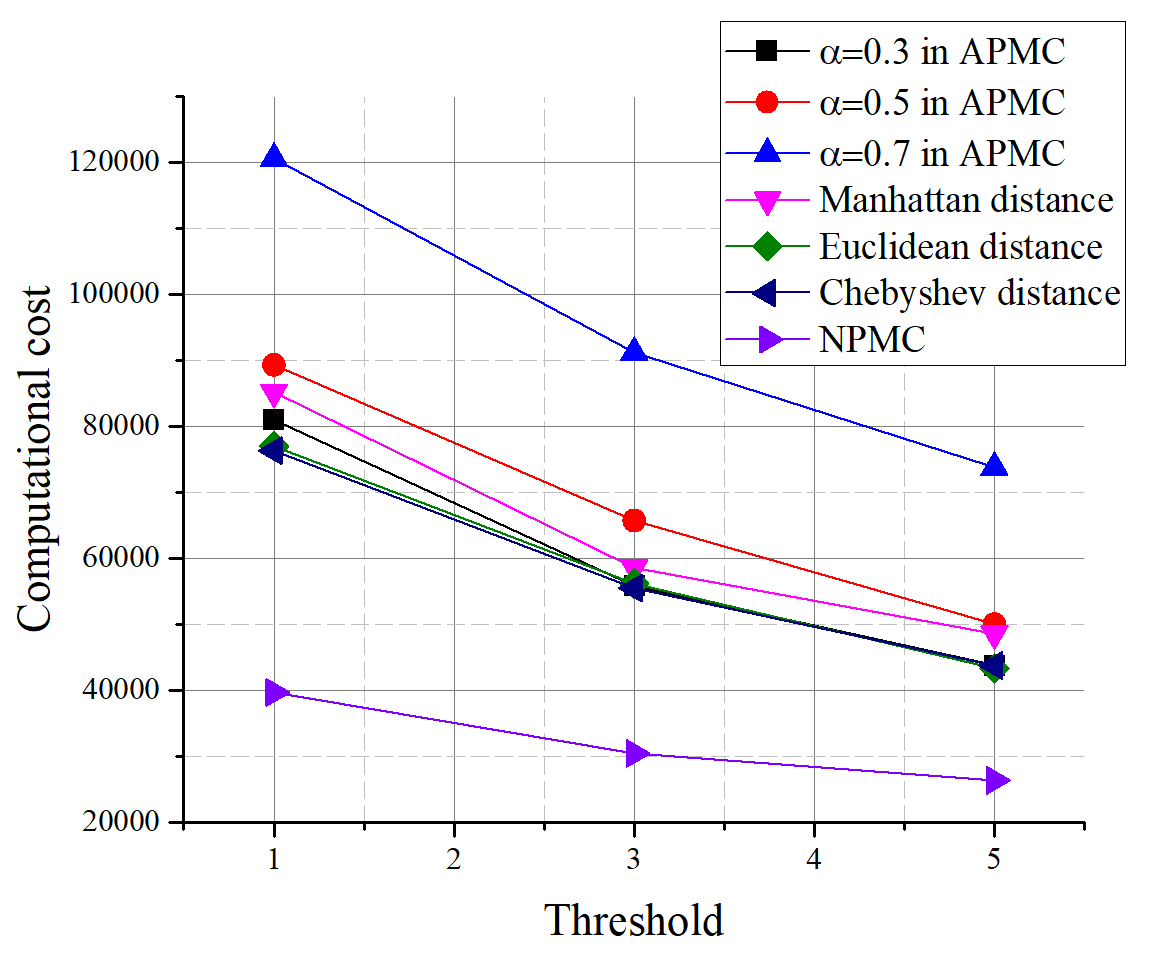
\includegraphics[width=0.8\textwidth]{fig/bench-cost.png}
    \caption{The computational cost of benchmark}
    \label{fig:bench_cost}
\end{figure}

\subsection{Flowchart of proposed method}
The flowchart of proposed framework as shown in Fig.\ref{fig:flowchar} is as follows:
\begin{enumerate}[Step 1:]
    \item Sampling: Sample based on PMC rule (In the first iteration, sample from given distribution. In other iterations, sample from last particles). Determine the distance of summary statistic using heat solver (superposition for linear issue, CA for nonlinear issue) and the tolerance value based on  \ref{eq:Euc}. Calculate the samples' weights
    \item Inheriting: inherit the samples with $d<\varepsilon_t$ from last particle
    \item Replenishing: Sample and accept with $d<\varepsilon_t$. Calculate the samples' weights and variance
    \item Next iteration: Go back to step 1 until $\varepsilon_t<\varepsilon_s$
\end{enumerate}

\begin{figure}
    \centering
    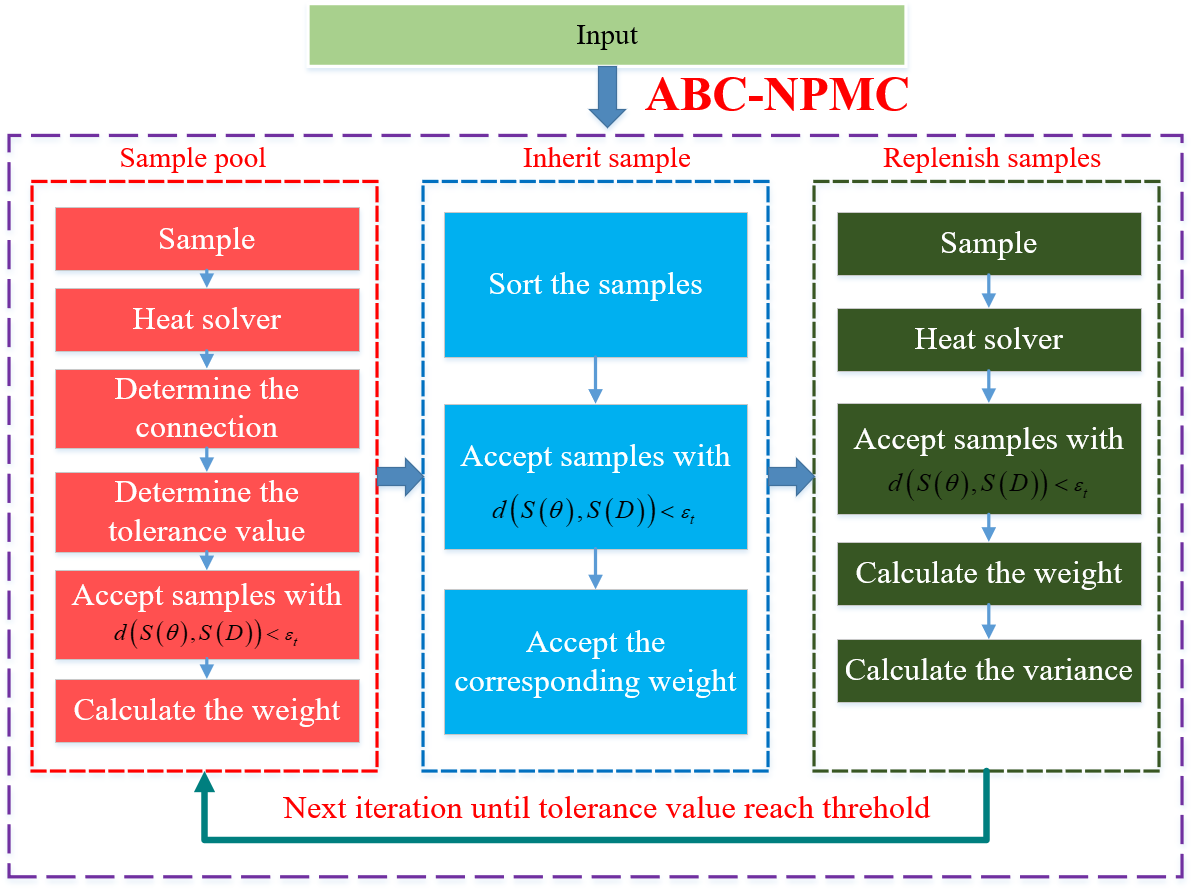
\includegraphics[width=0.98\textwidth]{./fig/flowchart.png}
    \caption{The flowchart of proposed framework}
    \label{fig:flowchar}
\end{figure}

\section{Numerical examples}
In this section, two examples including linear and nonlinear dynamic IHCPs are presented to examine the efficiency and the accuracy of the suggested methods, respectively. Since among four boundary conditions, Neumann boundary and Robin boundary conditions are the most widely used, we mainly focus on these two kinds of boundary conditions.

\subsection{Linear case}
\textcolor{red}{In this case, the heat conductivity coefficient is $k = 30W/(m\cdot ^\circ C)$. The $h_c$ and $T_\infty$ of the Robin boundary condition are given as $50W/m^2\cdot K$ and $30^{\circ}C$. The Neumann boundary condition at left and bottom are piecewise linear functions. The interests of this case is to reconstruct the heat flux of Neumann boundary condition based on the observations. Thus, these leads to a linear dynamic forward problem. The inverse of tangent matrix will be determined before calculation. The geometry are meshed as 613 nodes and 1022 triangle elements. After 210 iterate, the forward problem convergent as shown in Fig.\ref{fig:linearcase}. With superposition, it only take 0.26s.} 
 
 \begin{figure}
    \centering
    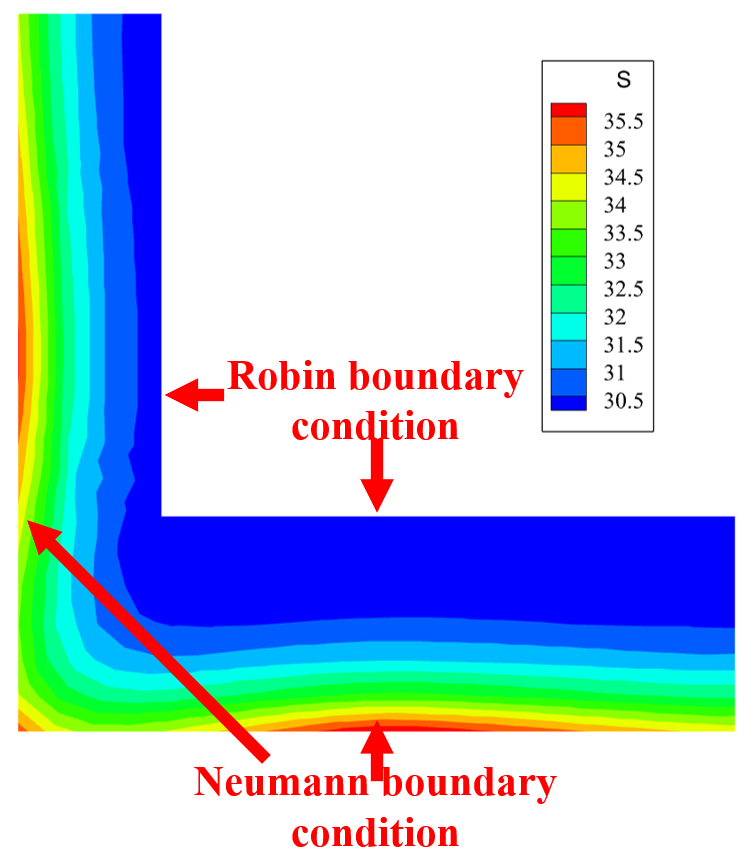
\includegraphics[width = 0.6\textwidth]{fig/case1-geo.png}
    \caption{The geometry and boundary condition of linear case}
    \label{fig:linearcase}
\end{figure}

 \textcolor{red}{According to Ref.\cite{wang2004bayesian}, the heat flux function can be discretized as}

\begin{equation}
    q(x) = \sum_{i=1}^m \theta_i w_i(x)
    \label{eq:functionheatflux}
\end{equation}

\noindent \textcolor{red}{where $w_i$'s are basis function. In this setting, if the weights $\theta_i$'s are determined, the function of heat flux can be reconstructed. With RS-HDMR the sensitivities of $\theta$'s are presented in Table.\ref{tab:sensi_case1}. Based on it, no parameters are filters in this case.}

\begin{table}[]
    \centering
    \caption{The sensitivities of $\theta$s}
    \begin{tabular}{c c c c c c c}
        \hline
         parameter & $\theta_{1,l}$ & $\theta_{2,l}$ & $\theta_{3,l}$ &$\theta_{1,b}$ & $\theta_{2,b}$ & $\theta_{3,b}$ \\
         \hline
         value & 0.2059 & 0.1746 & 0.1392 & 0.2082 & 0.1474 & 0.1217\\
        
         \hline
    \end{tabular}
    \label{tab:sensi_case1}
\end{table}

\textcolor{red}{Comprehensive comparison between traditional IHCP were presented in \cite{mocerino2018filtered, wang2004bayesian}. Here, the traditional Bayesian method with Markov chain Monte Carlo (MCMC) sampling is used to prove the performance of ABC. In this case, the temperature field on the surface are used as observations. Currently, the non-destructive such as infrared thermography which has been widely used can detect the temperature field of the surface. There are 613 observations. It should be noted that in Bayesian method, 613 observations are computational prohibited. Therefore, 40 observations are used in Bayesian method. Gaussian white noise with $\sigma=0.1$ and $0.5$ is added to the observations as uncertainties\cite{doltsinis2001ordinary}, respectively. }

\textcolor{red}{In Bayesian method, 50000 samples are generated by MCMC. While in ABC, 40 iterations are calculated. The tolerance values in ABC calculation are presented in Fig.\ref{fig:convergence}. It can be found that the tolerance values approach constant after 40 iterations. It means that the ABC reaches convergence. The convergent value is different for different noise. 83605 forward problem calculations are implemented for $\sigma=0.1$ with 40 iterations. 83587 forward problem calculations are implemented for $\sigma=0.5$ with 40 iterations.} 

\begin{figure}
    \centering
    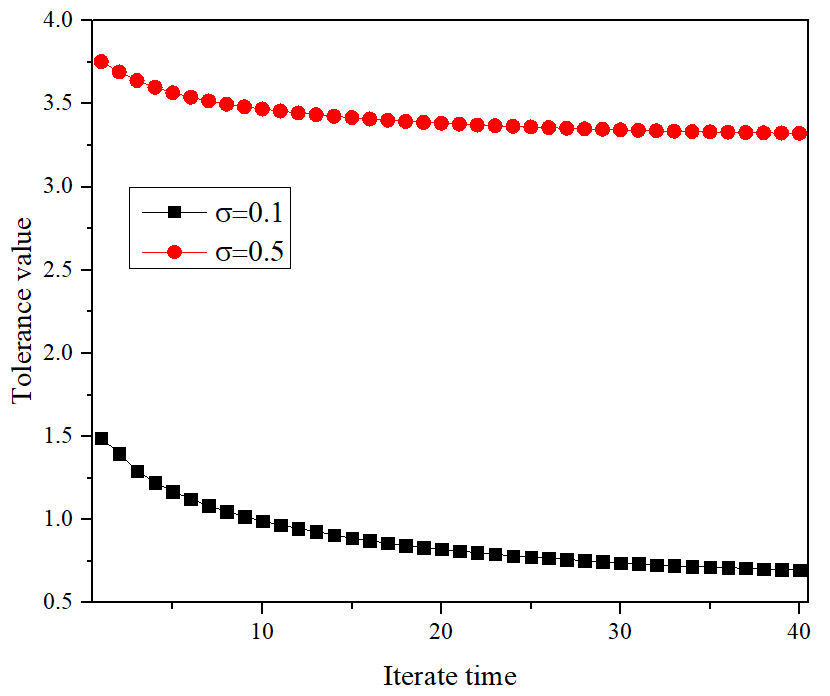
\includegraphics[width=0.6\textwidth]{fig/convergence.png}
    \caption{The tolerance value in ABC calculation}
    \label{fig:convergence}
\end{figure}

\textcolor{red}{The reconstructions of the heat flux function with Bayesian method and ABC are presented in Fig.\ref{fig:resultofflux}. At first, three weights are used for each piecewise linear heat flux function. The means and standard deviations of Bayesian posteriors and ABC posteriors are listed in Table.\ref{tab:mean_case1} and \ref{tab:std_case1}. The ABC posteriors with $\sigma=0.1$ are presented in Fig.\ref{fig:appro_post_case1}. From Fig.\ref{fig:resultofflux} and Table.\ref{tab:mean_case1}, it can be found that Bayesian method can obtain a more accurate inference. However, the predictions of ABC (the purple and green line) are still acceptable. From Table.\ref{tab:std_case1}, it can be found that in this case, the standard deviations of ABC can be smaller than that of Bayesian method. This means the uncertainty \cite{doltsinis2001ordinary} of ABC posteriors is less than that of Bayesian method. This is because only part of observations are used in Bayesian method. In Bayesian method, more observations result in smaller posterior standard deviations. ABC shows a strong ability of using all observations and obtain a very flexible and feasible performance.}

\begin{figure}
    \centering
    \centering
    \subfloat[Heat flux function at left]{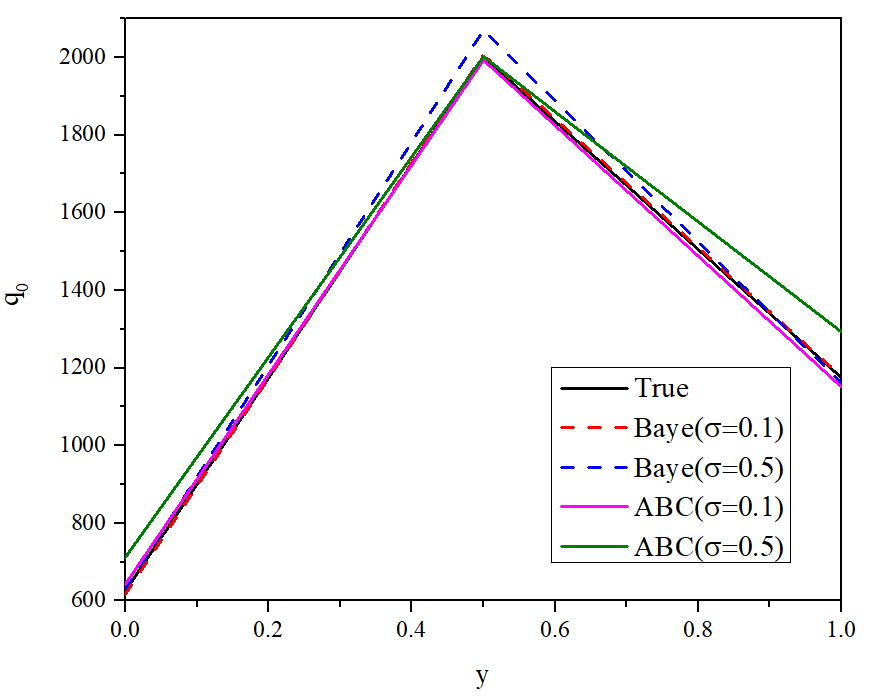
\includegraphics[width=0.45\textwidth]{./fig/resultofleft.png}}
    \subfloat[Heat flux function at bottom]{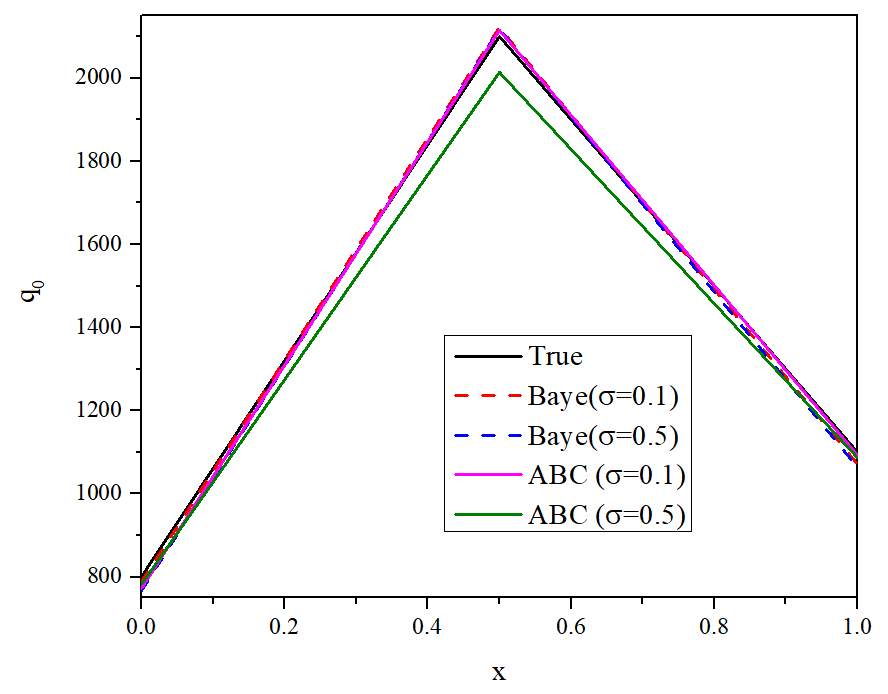
\includegraphics[width=0.45\textwidth]{./fig/resultofright.png}}
    \caption{The reconstruction of heat flux}
    \label{fig:resultofflux}
\end{figure}

\begin{table}[]
    \centering
    \caption{The means of Bayesian posteriors and approximate posteriors}
    \begin{tabular}{c c c c c c c c}
        \hline
         parameter & $\theta_{1,l}$ & $\theta_{2,l}$ & $\theta_{3,l}$ &$\theta_{1,b}$ & $\theta_{2,b}$ & $\theta_{3,b}$ & error \\
         \hline
         Truth &900 & 2000 & 1340 & 1060 & 2100 & 1300 & \\
         Baye( $\sigma=0.1$ ) & 894.6 & 2007.7 & 1344.4 & 1054.5 & 2121.5 & 1281.4 & 0.12\%\\
         Baye( $\sigma=0.5$ ) & 919.0 & 2069.9 & 1343.0 & 1037.1 & 2117.8 & 1274.6 & 0.53\%\\
         ABC( $\sigma=0.1$ ) & 912.9 & 1993.2 & 1319.5 & 1040.8 & 2114.6 & 1297.3 & 0.20\%\\
         ABC( $\sigma=0.5$ ) & 970.3 & 2001.9 & 1434.7 & 1028.0 & 2013.6 & 1272.3 & 0.78\%\\
         \hline
    \end{tabular}
    \label{tab:mean_case1}
\end{table}

\begin{table}[]
    \centering
    \caption{The standard deviation of Bayesian posteriors and approximate posteriors}
    \begin{tabular}{c c c c c c c}
        \hline
         parameter & $\theta_{1,l}$ & $\theta_{2,l}$ & $\theta_{3,l}$ &$\theta_{1,b}$ & $\theta_{2,b}$ & $\theta_{3,b}$ \\
         \hline
         Baye( $\sigma=0.1$ ) & 16.36 & 16.34 & 14.63 & 16.34 & 15.15 & 14.62\\
         Baye( $\sigma=0.5$ ) & 33.53&50.43&50.33&32.67&69.77&53.88\\
         ABC( $\sigma=0.1$ ) & 15.28 & 15.10 & 13.50 & 15.44 & 14.04 & 13.55\\
         ABC( $\sigma=0.5$ ) & 29.16 & 32.47 & 28.61 & 30.00 & 31.55 & 29.87\\
         \hline
    \end{tabular}
    \label{tab:std_case1}
\end{table}

\begin{figure}
    \centering
    \subfloat[$\theta_{1,l}$]{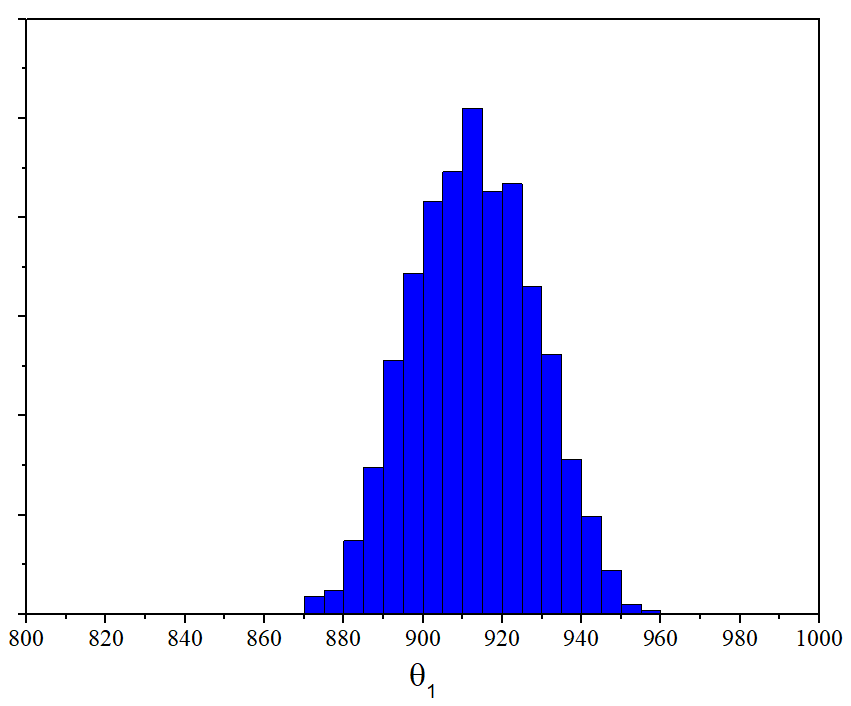
\includegraphics[width=0.45\textwidth]{./fig/Noise01_appro_1.png}}
    \subfloat[$\theta_{2,l}$]{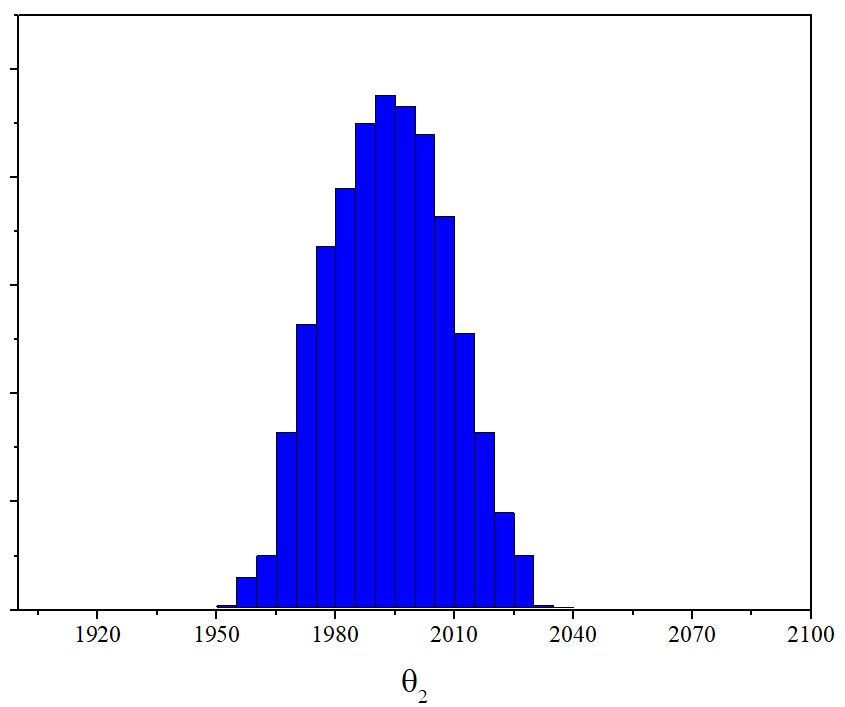
\includegraphics[width=0.45\textwidth]{./fig/Noise01_appro_2.png}}
    
    \subfloat[$\theta_{3,l}$]{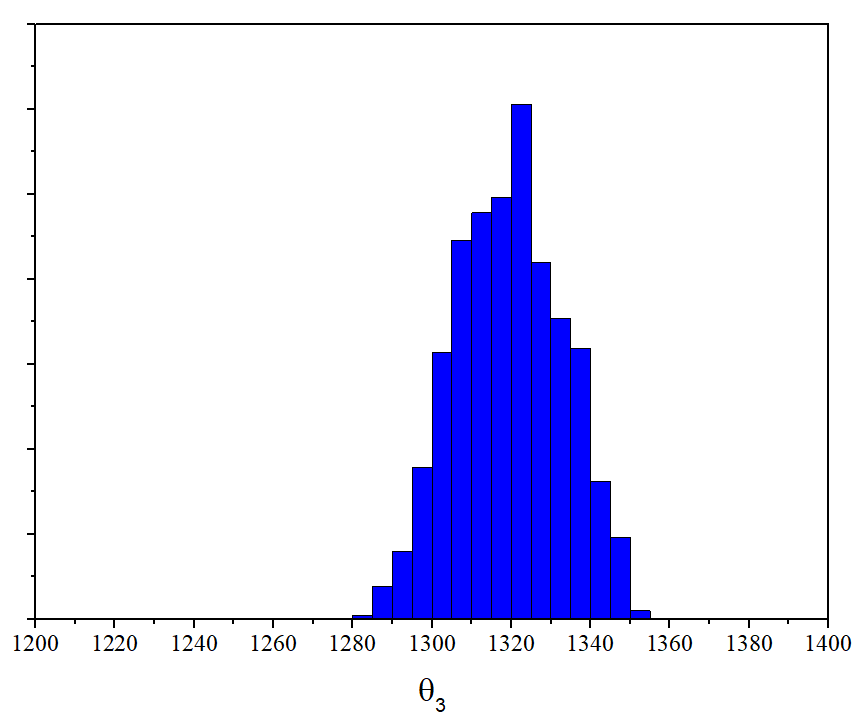
\includegraphics[width=0.45\textwidth]{./fig/Noise01_appro_3.png}}
    \subfloat[$\theta_{1,b}$]{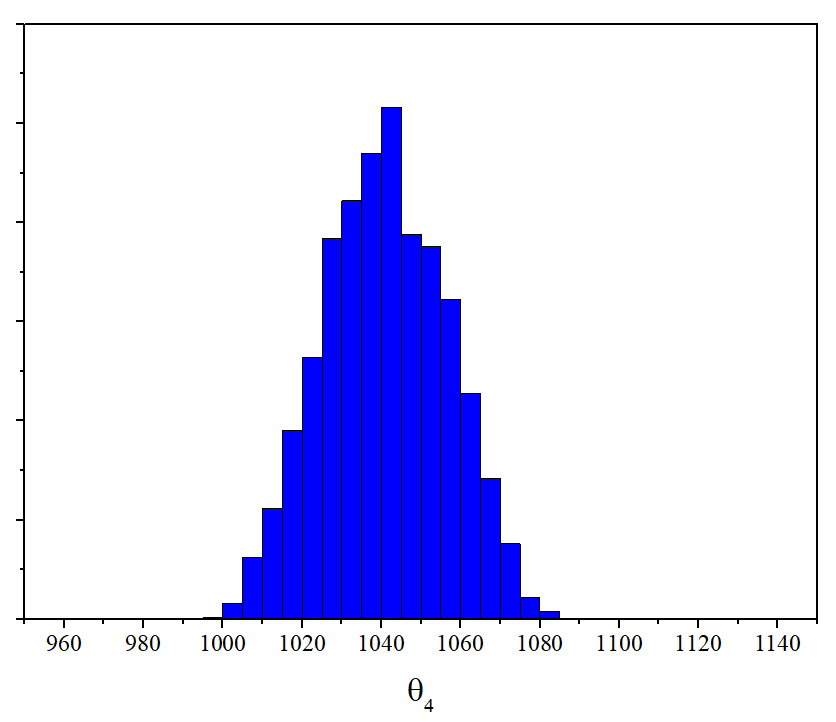
\includegraphics[width=0.45\textwidth]{./fig/Noise01_appro_4.png}}
    
    \subfloat[$\theta_{2,b}$]{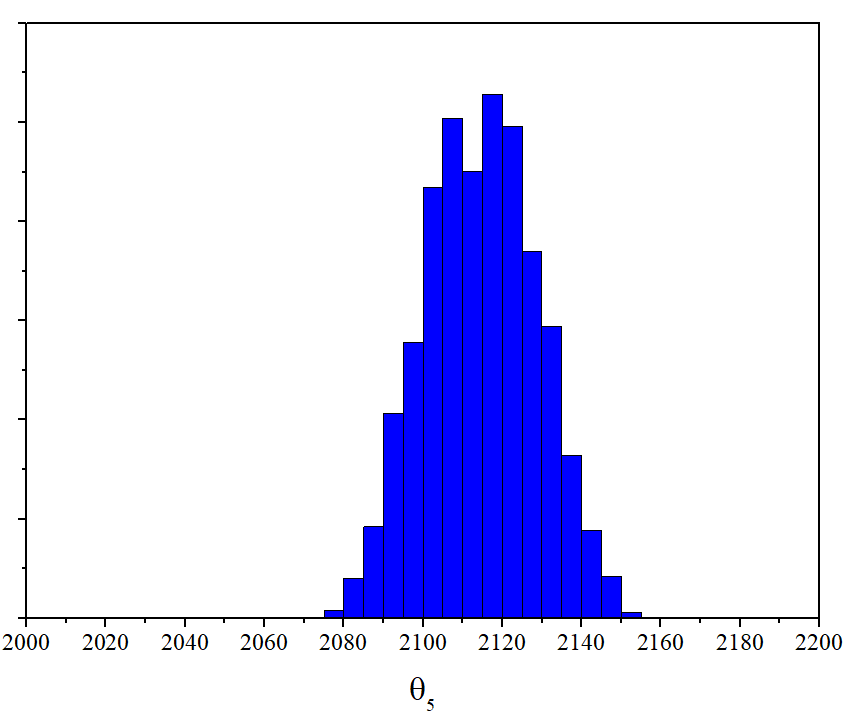
\includegraphics[width=0.45\textwidth]{./fig/Noise01_appro_5.png}}
    \subfloat[$\theta_{3,b}$]{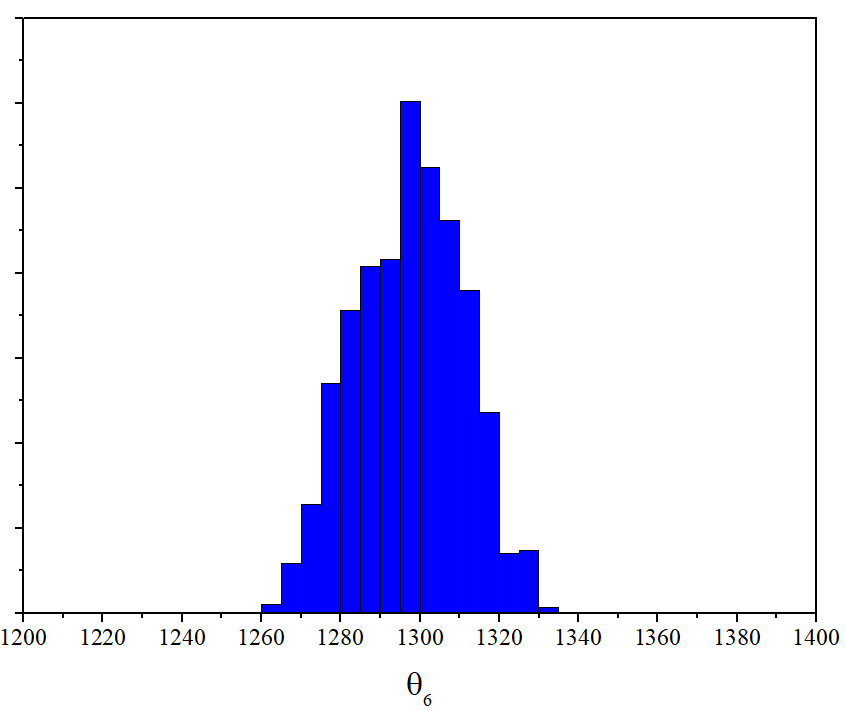
\includegraphics[width=0.45\textwidth]{./fig/Noise01_appro_6.png}}
    \caption{The ABC posteriors with $\sigma=0.1$}
    \label{fig:appro_post_case1}
\end{figure}

\textcolor{red}{In practice, the heat flux function is more complex. Therefore more weights $\theta$'s in Eq.~\ref{eq:functionheatflux} are needed. Here we add the number of $\theta$'s and 5 $\theta$'s are used for each heat flux function to test the ability of ABC for more complex function. Here, $\sigma=0.1$ is used. The results are presented in Fig.\ref{fig:resultofflux10}. It can be found ABC can obtain a very good prediction for high dimensional issue such as 10.}

\begin{figure}
    \centering
    \centering
    \subfloat[Heat flux function at left]{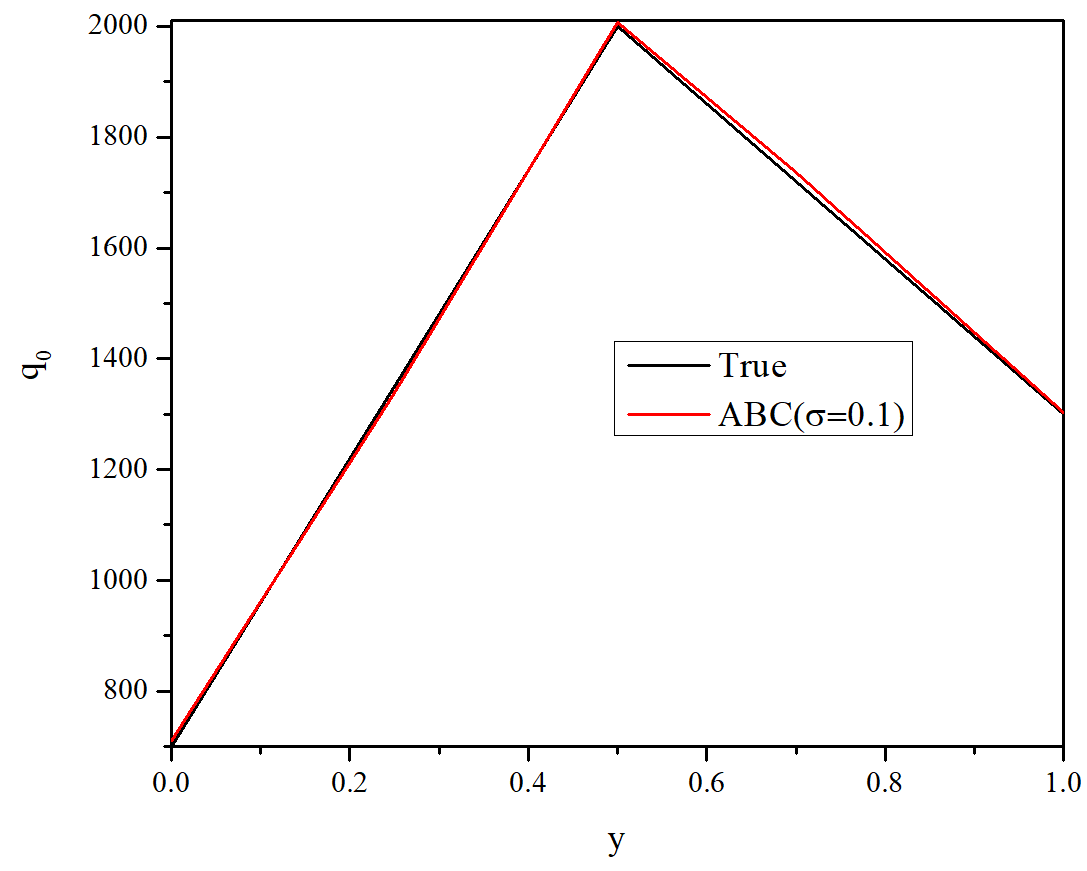
\includegraphics[width=0.45\textwidth]{./fig/left_10.png}}
    \subfloat[Heat flux function at bottom]{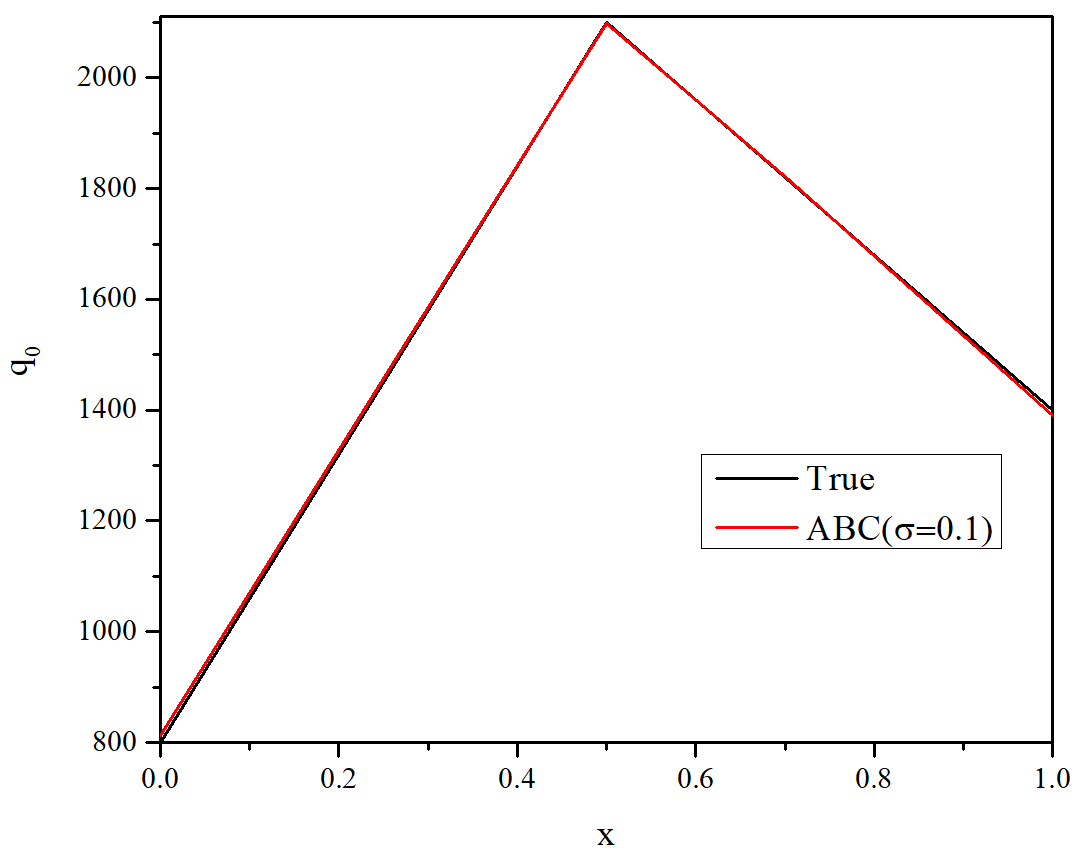
\includegraphics[width=0.45\textwidth]{./fig/right_10.png}}
    \caption{The reconstruction of heat flux function for more $\theta$'s}
    \label{fig:resultofflux10}
\end{figure}

\subsection{Nonlinear case}
In this section, a 3D heat sink is presented to demonstrate the efficiency of proposed method. Three boundary conditions are applied as shown in Fig.\ref{fig:3Dheatsink}. The 3D heat sink is meshed with 5,741 nodes and 22,927 tetrahedron elements. Some general parameters are listed in Table.\ref{tab:para_case2}. The observations are the temperature on the front and back surface at 10s, 20s, 30s generated with the parameters shown in Table.\ref{tab:unkownpara}. There are 388 observations in this case. Gaussian white noise with $\sigma=0.1$ is added to the temperature as the uncertainties such as measurement error and so on. 

\begin{figure}
    \centering
    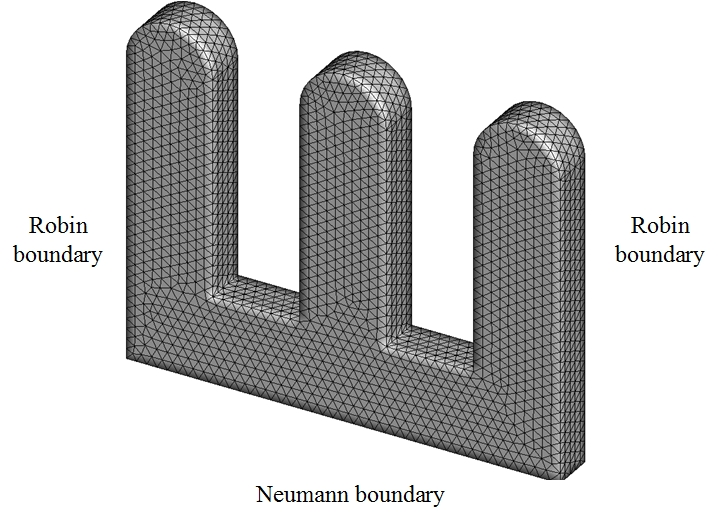
\includegraphics[width=0.7\textwidth]{fig/3Dheatsink.png}
    \caption{The mesh and boundary condition of 3D heat sink}
    \label{fig:3Dheatsink}
\end{figure}

\begin{table}[]
    \centering
    \caption{The geometry and physical parameters}
    \begin{tabular}{c c c c}
        \hline
         Parameters &  $k$ & $c$ & $\rho$\\
         \hline
         Value &  $(30+0.1T)W/m\cdot ^{\circ} C$ & $50 J/Kg \cdot K$ & $300 Kg/m^3$\\
         \hline
    \end{tabular}
    \label{tab:para_case2}
\end{table}

\begin{table}[]
    \centering
    \caption{The parameters of boundary to generate observations}
    \begin{tabular}{c c c c c c}
        \hline
         Boundary &  \multicolumn{2}{c}{ Left Robin } & \multicolumn{2}{c}{Right Robin } & Neumann \\
         \hline
         Unknowns &  $h_c$ & $T_\infty$ & $h_c$ & $T_\infty$ & $q_0$\\
         Value  &  $250 W/m^2 \cdot ^{\circ}C$ & $80^{\circ}C$ & $200 W/m^2 \cdot^{\circ}C$ & $100^{\circ}C$ & $-1000W/m^2$\\
         \hline
    \end{tabular}
    \label{tab:unkownpara}
\end{table}

Before determining determination of the unknowns, the accuracy and efficiency of reanalysis based dynamic heat conduction solver are tested. The temperature fields solved by FEM and reanalysis at 10s, 20s and 30s are presented in Fig.\ref{fig:FEM_CA}. The temperature values of some specified nodes are presented in Table.\ref{tab:com_FEM_CA}. The computational costs with FEM and CA method are listed in Table.. According to Table.\ref{tab:com_FEM_CA} and Fig.\ref{fig:FEM_CA}, it can be found that the difference between the temperature field solved by FEM and reanalysis is no more than 0.1\%. The one-time computational time of reanalysis is less than one fourth of that of FEM as shown in Table.\ref{tab:com_cost}. The total computational time of reanalysis is less than half of that of FEM. Thus, the CA reanalysis is rather efficient with high accuracy.

\begin{figure}
\centering
\subfloat[FEM result at 10s]{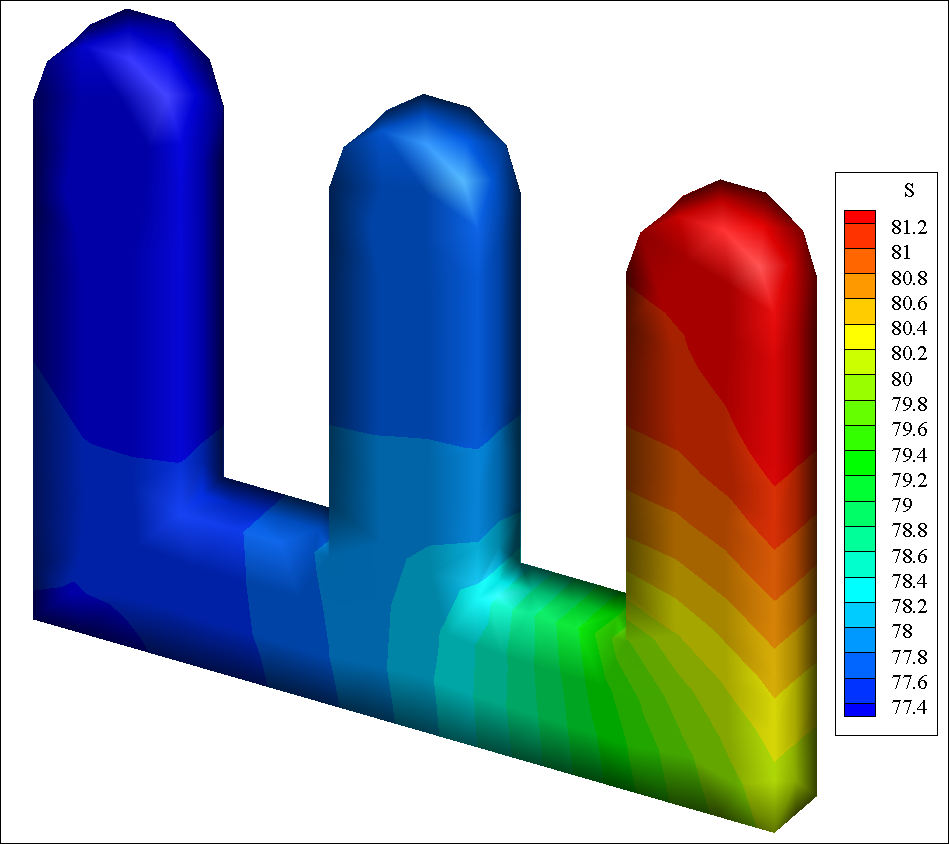
\includegraphics[width=0.45\textwidth]{./fig/FEM-step1.png}}
\subfloat[CA result at 10s]{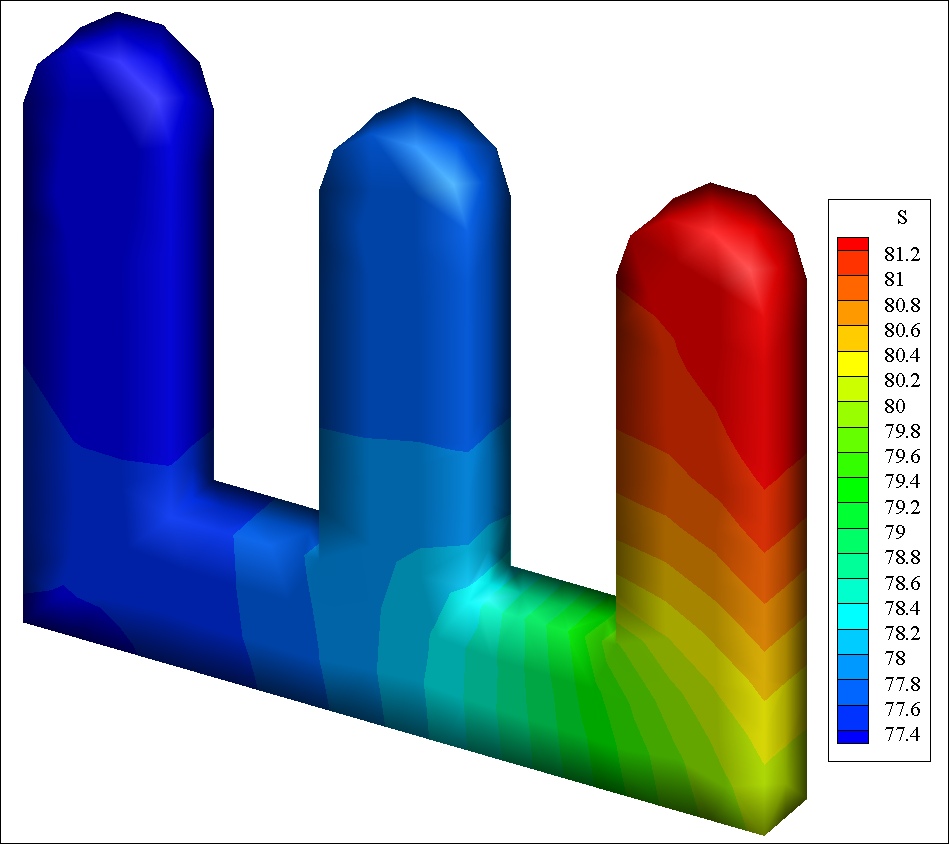
\includegraphics[width=0.45\textwidth]{./fig/CA-step1.png}}

\subfloat[FEM result at 20s]{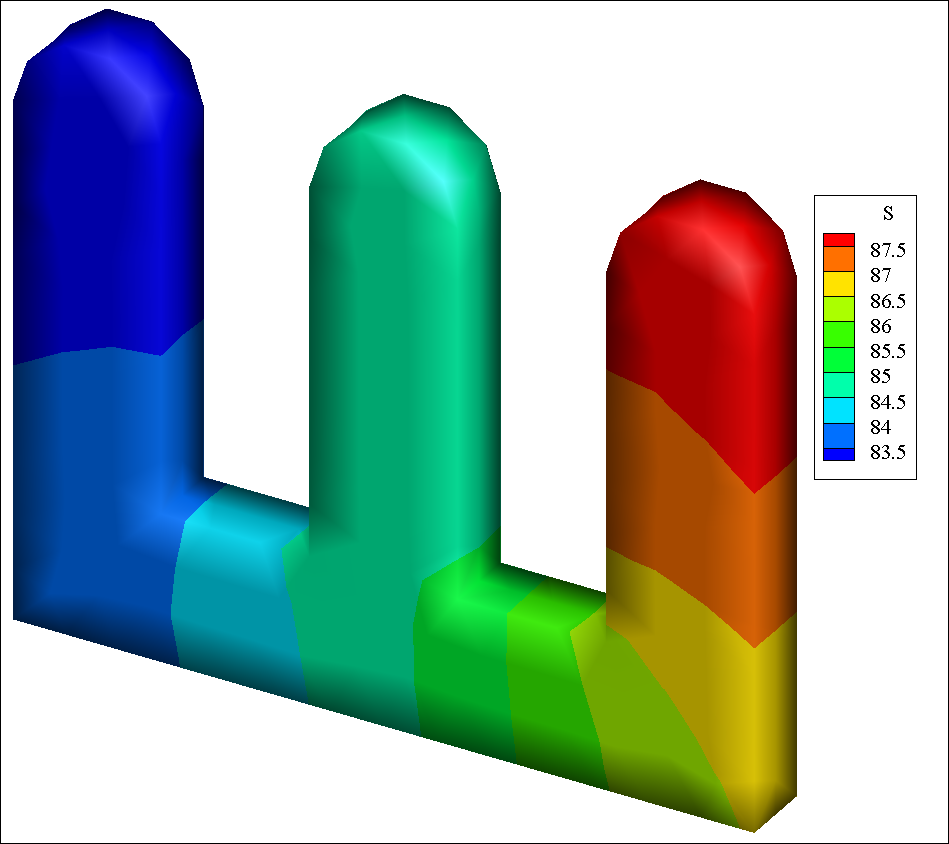
\includegraphics[width=0.45\textwidth]{./fig/FEM-step2.png}}
\subfloat[CA result at 20s]{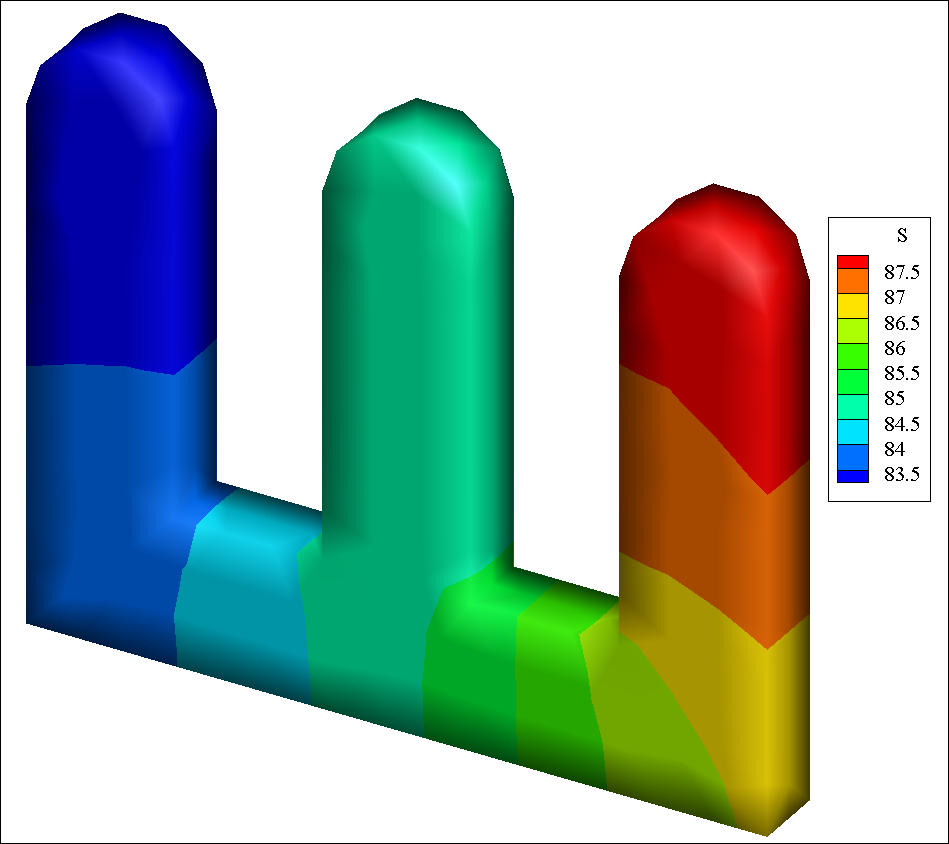
\includegraphics[width=0.45\textwidth]{./fig/CA-step2.png}}

\subfloat[FEM result at 30s]{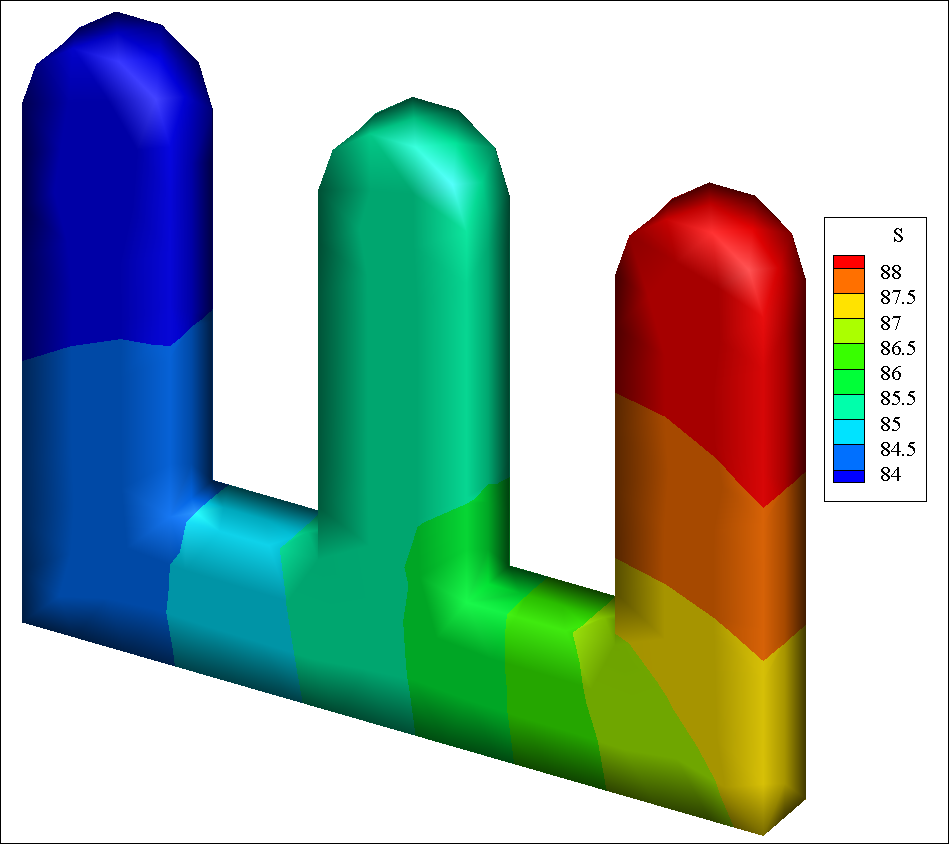
\includegraphics[width=0.45\textwidth]{./fig/FEM-step3.png}}
\subfloat[CA result at 30s]{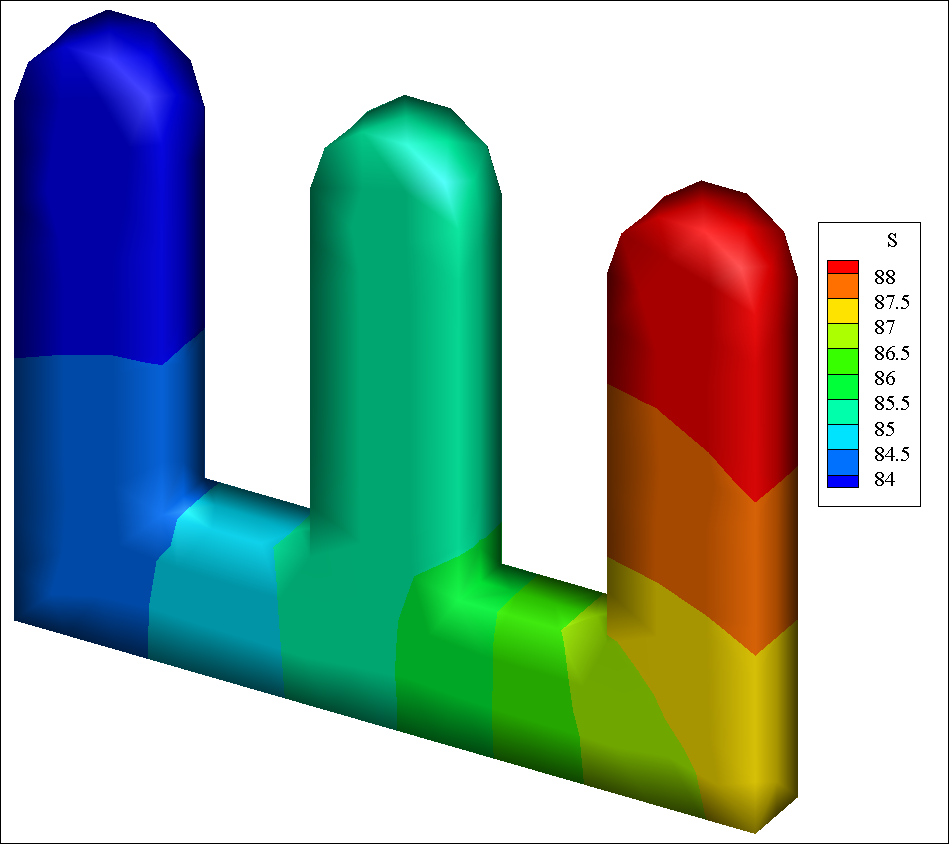
\includegraphics[width=0.45\textwidth]{./fig/CA-step3.png}}

\caption{The comparison of FEM and CA solver}
\label{fig:FEM_CA}
\end{figure}

\begin{table}[]
    \centering
    \caption{The comparison of accuracy of FEM and CA at some nodes }
    \begin{tabular}{c c c c c c c}
    \hline
         Node & \multicolumn{3}{c}{FEM } &  \multicolumn{3}{c}{CA} \\
         \cline{2-7}
         number & 10s & 20s & 30s & 10s & 20s & 30s\\
         \hline
         1	&77.3801&83.7227&84.2513&77.3802&83.6512&84.1765\\
        1001 & 77.6069 & 84.8525 & 85.4638 & 77.6064 & 84.6298 & 85.2177\\
        2001 & 78.6065 & 85.3854 & 85.9539 & 78.6069 & 85.4097 & 85.9772\\
        3001 & 81.0570 & 87.4184 & 87.9492 & 81.0568 & 87.4118 & 87.9403\\
        \hline
    \end{tabular}
    \label{tab:com_FEM_CA}
\end{table}

\begin{table}[]
    \centering
    \caption{The computational cost}
    \begin{tabular}{c c c}
    \hline
         Methods & FEM & CA method \\
         \hline
        Time of each iteration & 4.07s & 0.82s\\
        Simulation time & 88.3s & 34.6s\\
        \hline
    \end{tabular}
    \label{tab:com_cost}
\end{table}

According to the results, we found that all parameters except heat flux are sensitive to the increment $\Delta \mathbf{T}$  of temperature between 10s, 20s and 20s, 30s. The results of sensitive analysis are presented in Table.\ref{tab:case2-sensitive}. According to Table.\ref{tab:case2-sensitive}, it can be found that the sensitivity of heat flux is much smaller than the other parameters. Therefore, four parameters should be identified. The increment  $\Delta \mathbf{T}$ is used as the observations of IHCP.

\begin{table}[]
    \centering
    \caption{The sensitivity of unknown parameters}
    \begin{tabular}{c c c c c c}
        \hline
         Boundary &  \multicolumn{2}{c}{ Left Robin } & \multicolumn{2}{c}{Right Robin } & Neumann \\
         \hline
         Unknowns &  $h_c$ & $T_\infty$ & $h_c$ & $T_\infty$ & $q_0$\\
         Value  &  0.2308 & 0.3068 & 0.1093 & 0.3122 & 0.0022\\
         \hline
    \end{tabular}
    \label{tab:case2-sensitive}
\end{table}

Gaussian prior which the mean is $1.2\theta_{true}$ and standard deviation is $0.05_{true}$ are used as shown in Fig.11. 
The NPMC in \textbf{Algorithm 2} assisted by the dynamic reanalysis solver is implemented to identify the unknowns. Here, the $\varepsilon$ is predefined as $0.2$. After 14 iterations, the tolerance value reaches $0.2$. The approximate posteriors are presented in Fig.\ref{fig:post_3D}. The means and standard deviations of priors and approximate posteriors are presented in Table.\ref{tab:case-post-mean} and \ref{tab:case-post-std}. According to Table.\ref{tab:case-post-mean}-\ref{tab:case-post-std} and Figs.\ref{fig:post_3D}, it is clear that the means of approximate posteriors are close to the true value of unknowns. The standard deviations of approximate posteriors are much smaller than that of priors. The number of total computational samples is 29,600 and the parallel reanalysis \cite{wang2013parallel} is used. If the APMC is implemented, more simulations are needed. Moreover, if the FEM is utilized, the computational cost will be more than twice higher than that of reanalysis. It can be concluded that the ABC-NPMC assisted by reanalysis dynamic solver can obtain flexible and feasible results.

\begin{table}[]
    \centering
    \caption{The mean of prior and approximate posterior }
    \begin{tabular}{c c c c c}
        \hline
          &  \multicolumn{2}{c}{ Left Robin } & \multicolumn{2}{c}{Right Robin } \\
         \hline
         parameters &  $h_c$ & $T_\infty$ & $h_c$ & $T_\infty$ \\
         Priors  &  300 & 96 & 240 & 120 \\
         Posteriors  &  250.11 & 79.93 & 199.92 & 99.99 \\
         \hline
    \end{tabular}
    \label{tab:case-post-mean}
\end{table}

\begin{table}[]
    \centering
    \caption{The standard deviation of prior and approximate posterior }
    \begin{tabular}{c c c c c}
        \hline
          &  \multicolumn{2}{c}{ Left Robin } & \multicolumn{2}{c}{Right Robin } \\
         \hline
         parameters &  $h_c$ & $T_\infty$ & $h_c$ & $T_\infty$ \\
         Priors  &  12.5 & 4 & 10 & 5 \\
         Posteriors  & 4.01 & 1.59 & 2.97 & 2.56 \\
         \hline
    \end{tabular}
    \label{tab:case-post-std}
\end{table}

\begin{figure}
\centering
\subfloat[The Robin boundary condition at left]{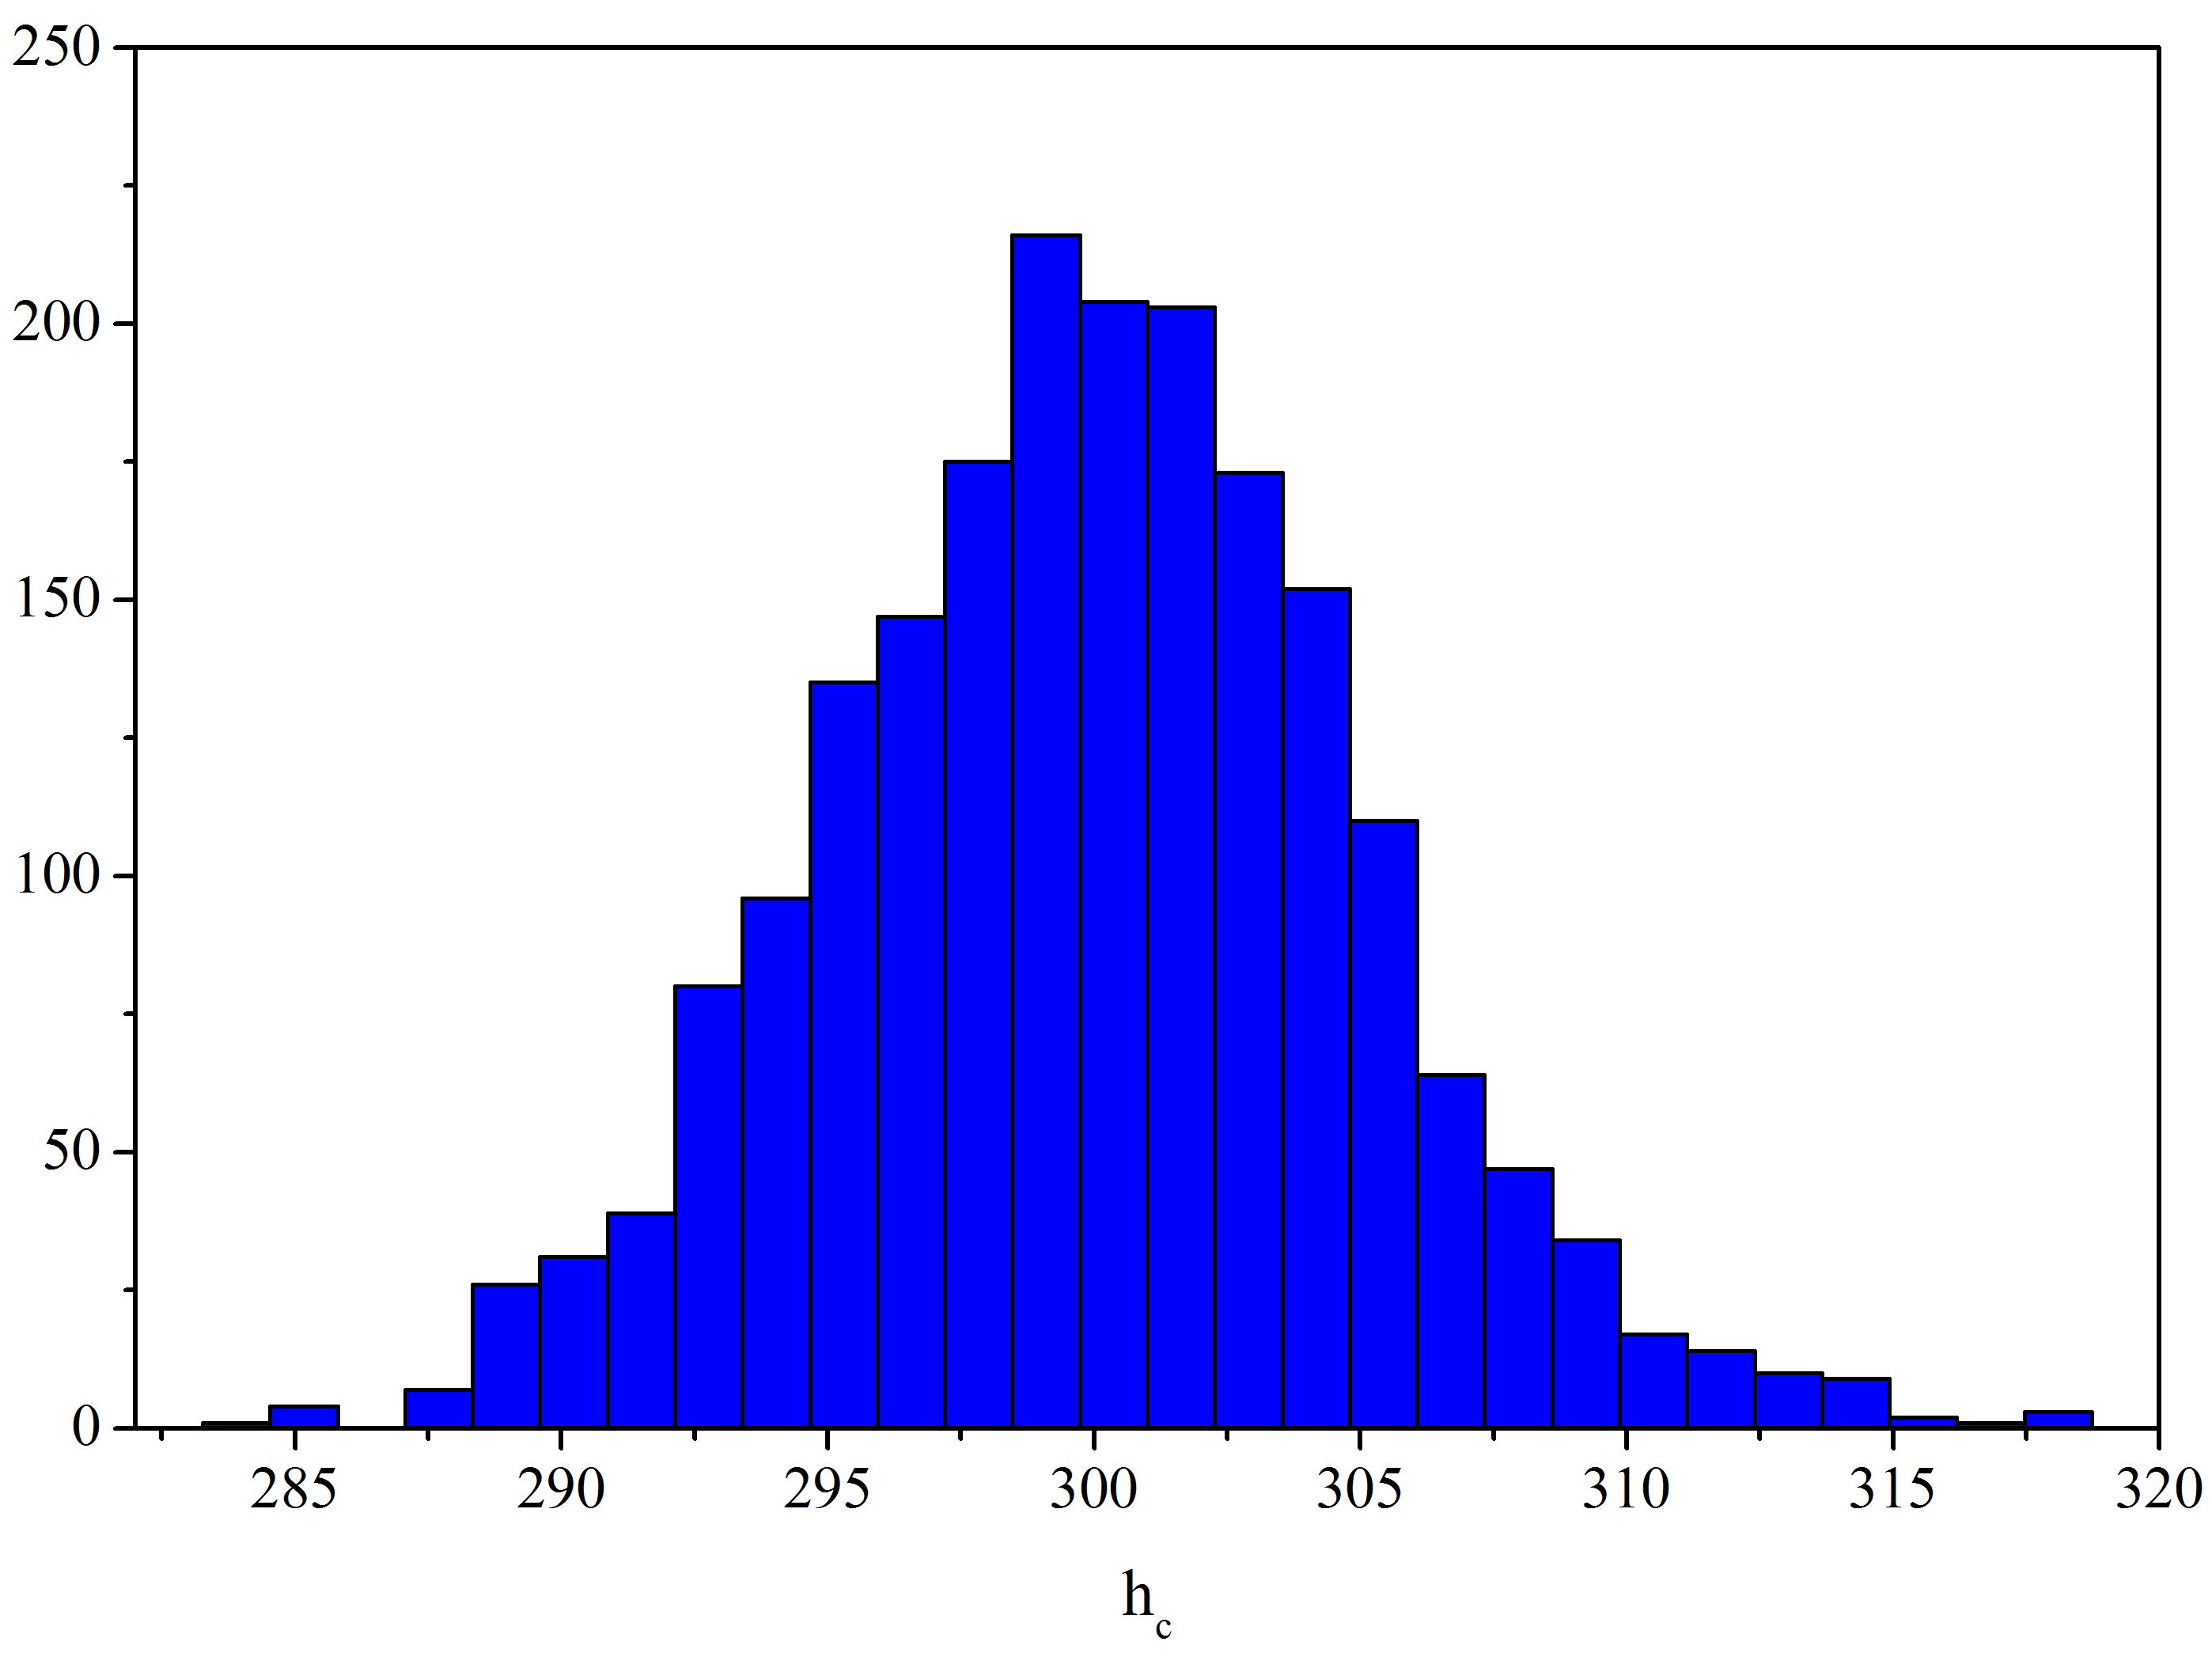
\includegraphics[width=0.45\textwidth]{./fig/Prior_left_hc.png}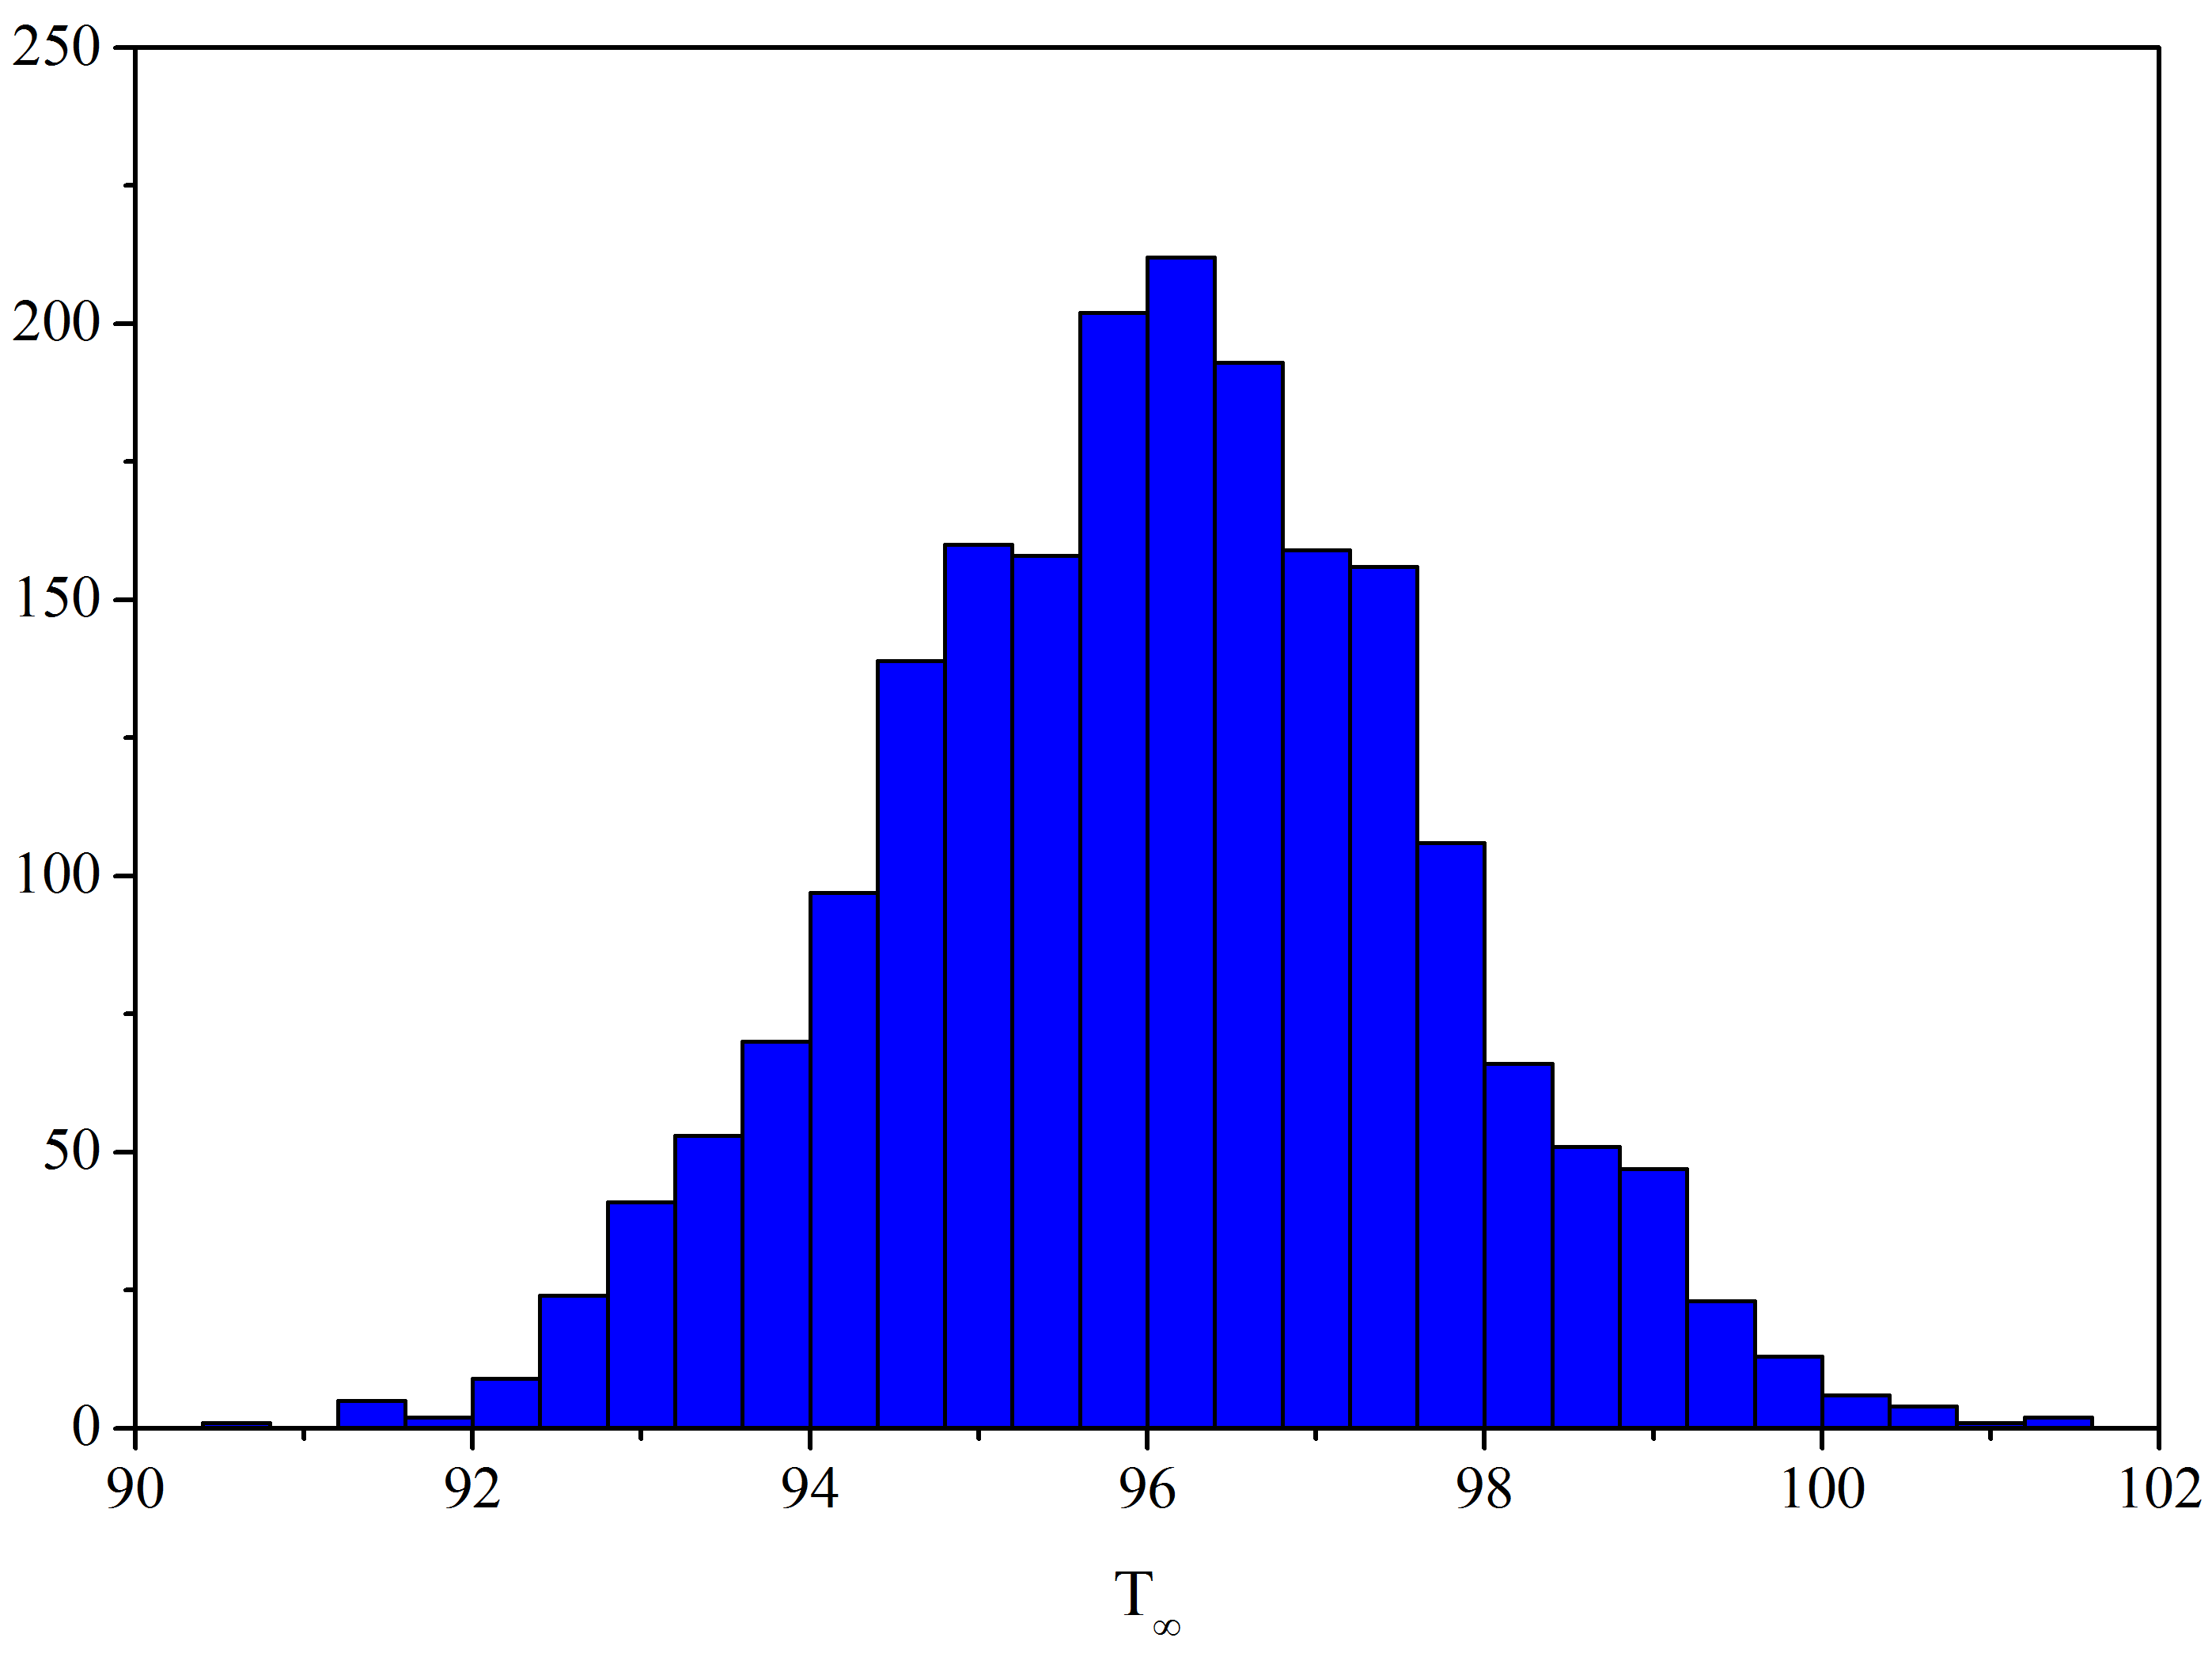
\includegraphics[width=0.45\textwidth]{./fig/Prior_left_T.png}}

\subfloat[The Robin boundary condition at right]{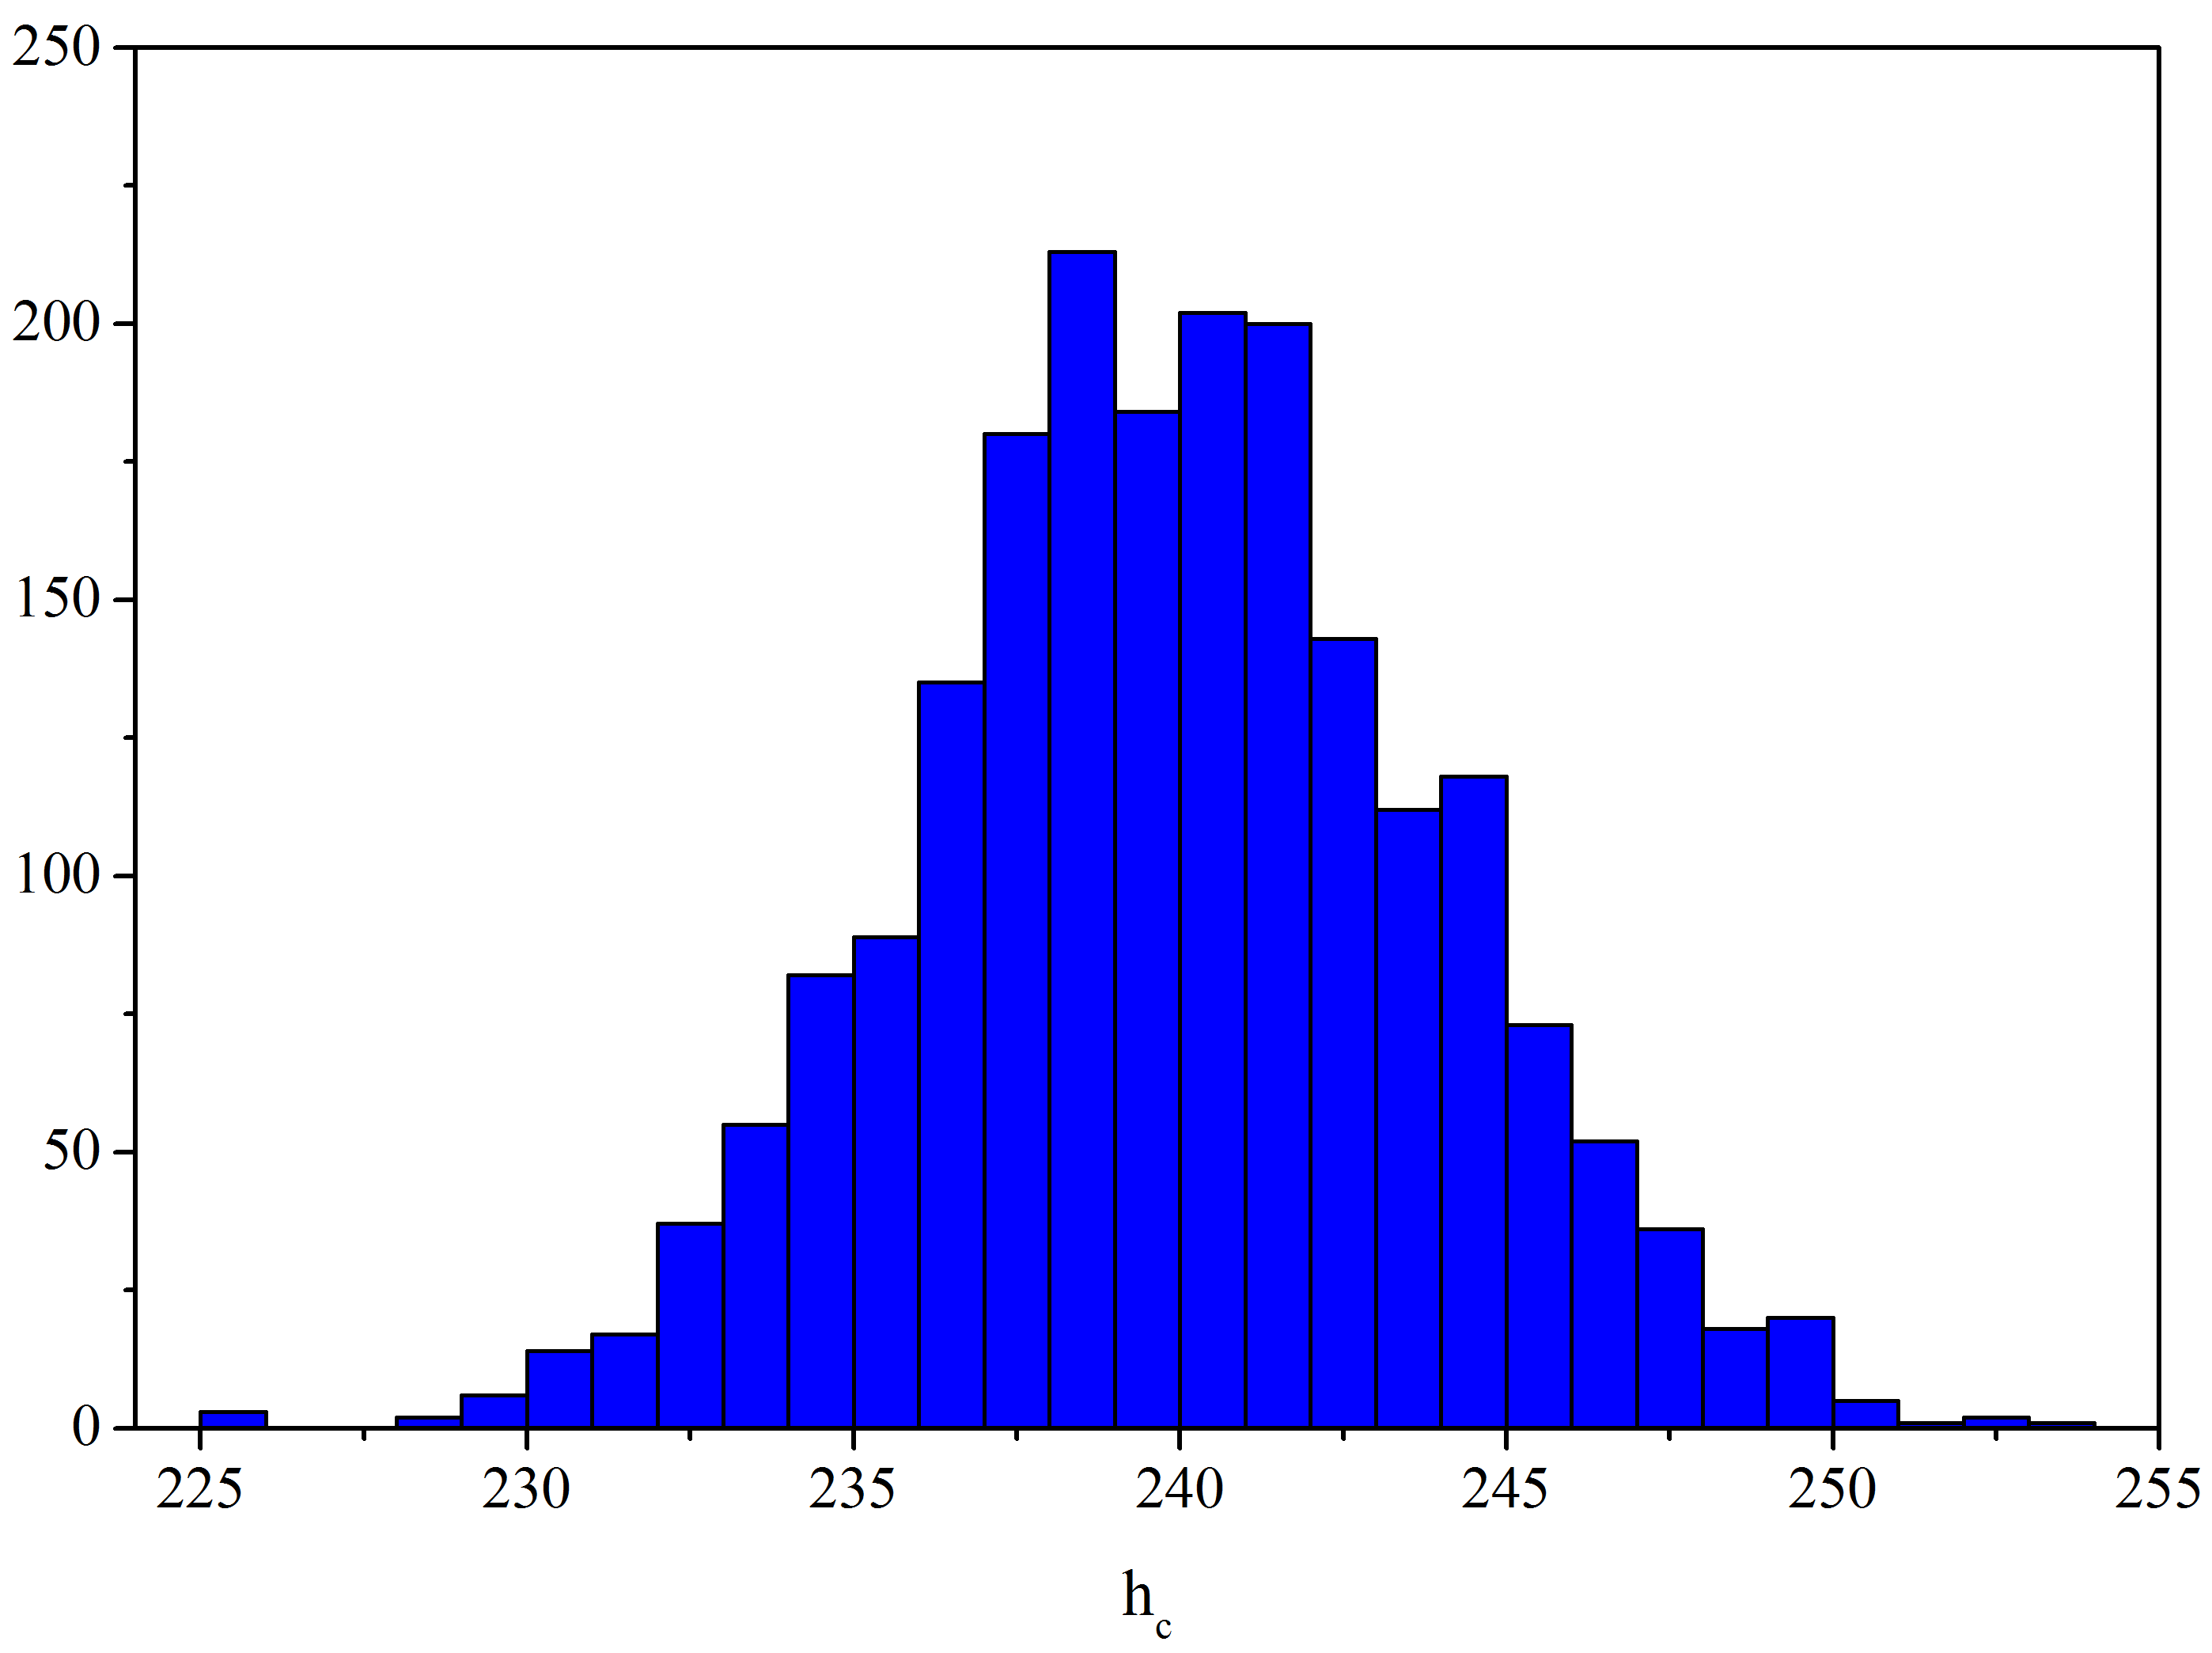
\includegraphics[width=0.45\textwidth]{./fig/Prior_right_hc.png}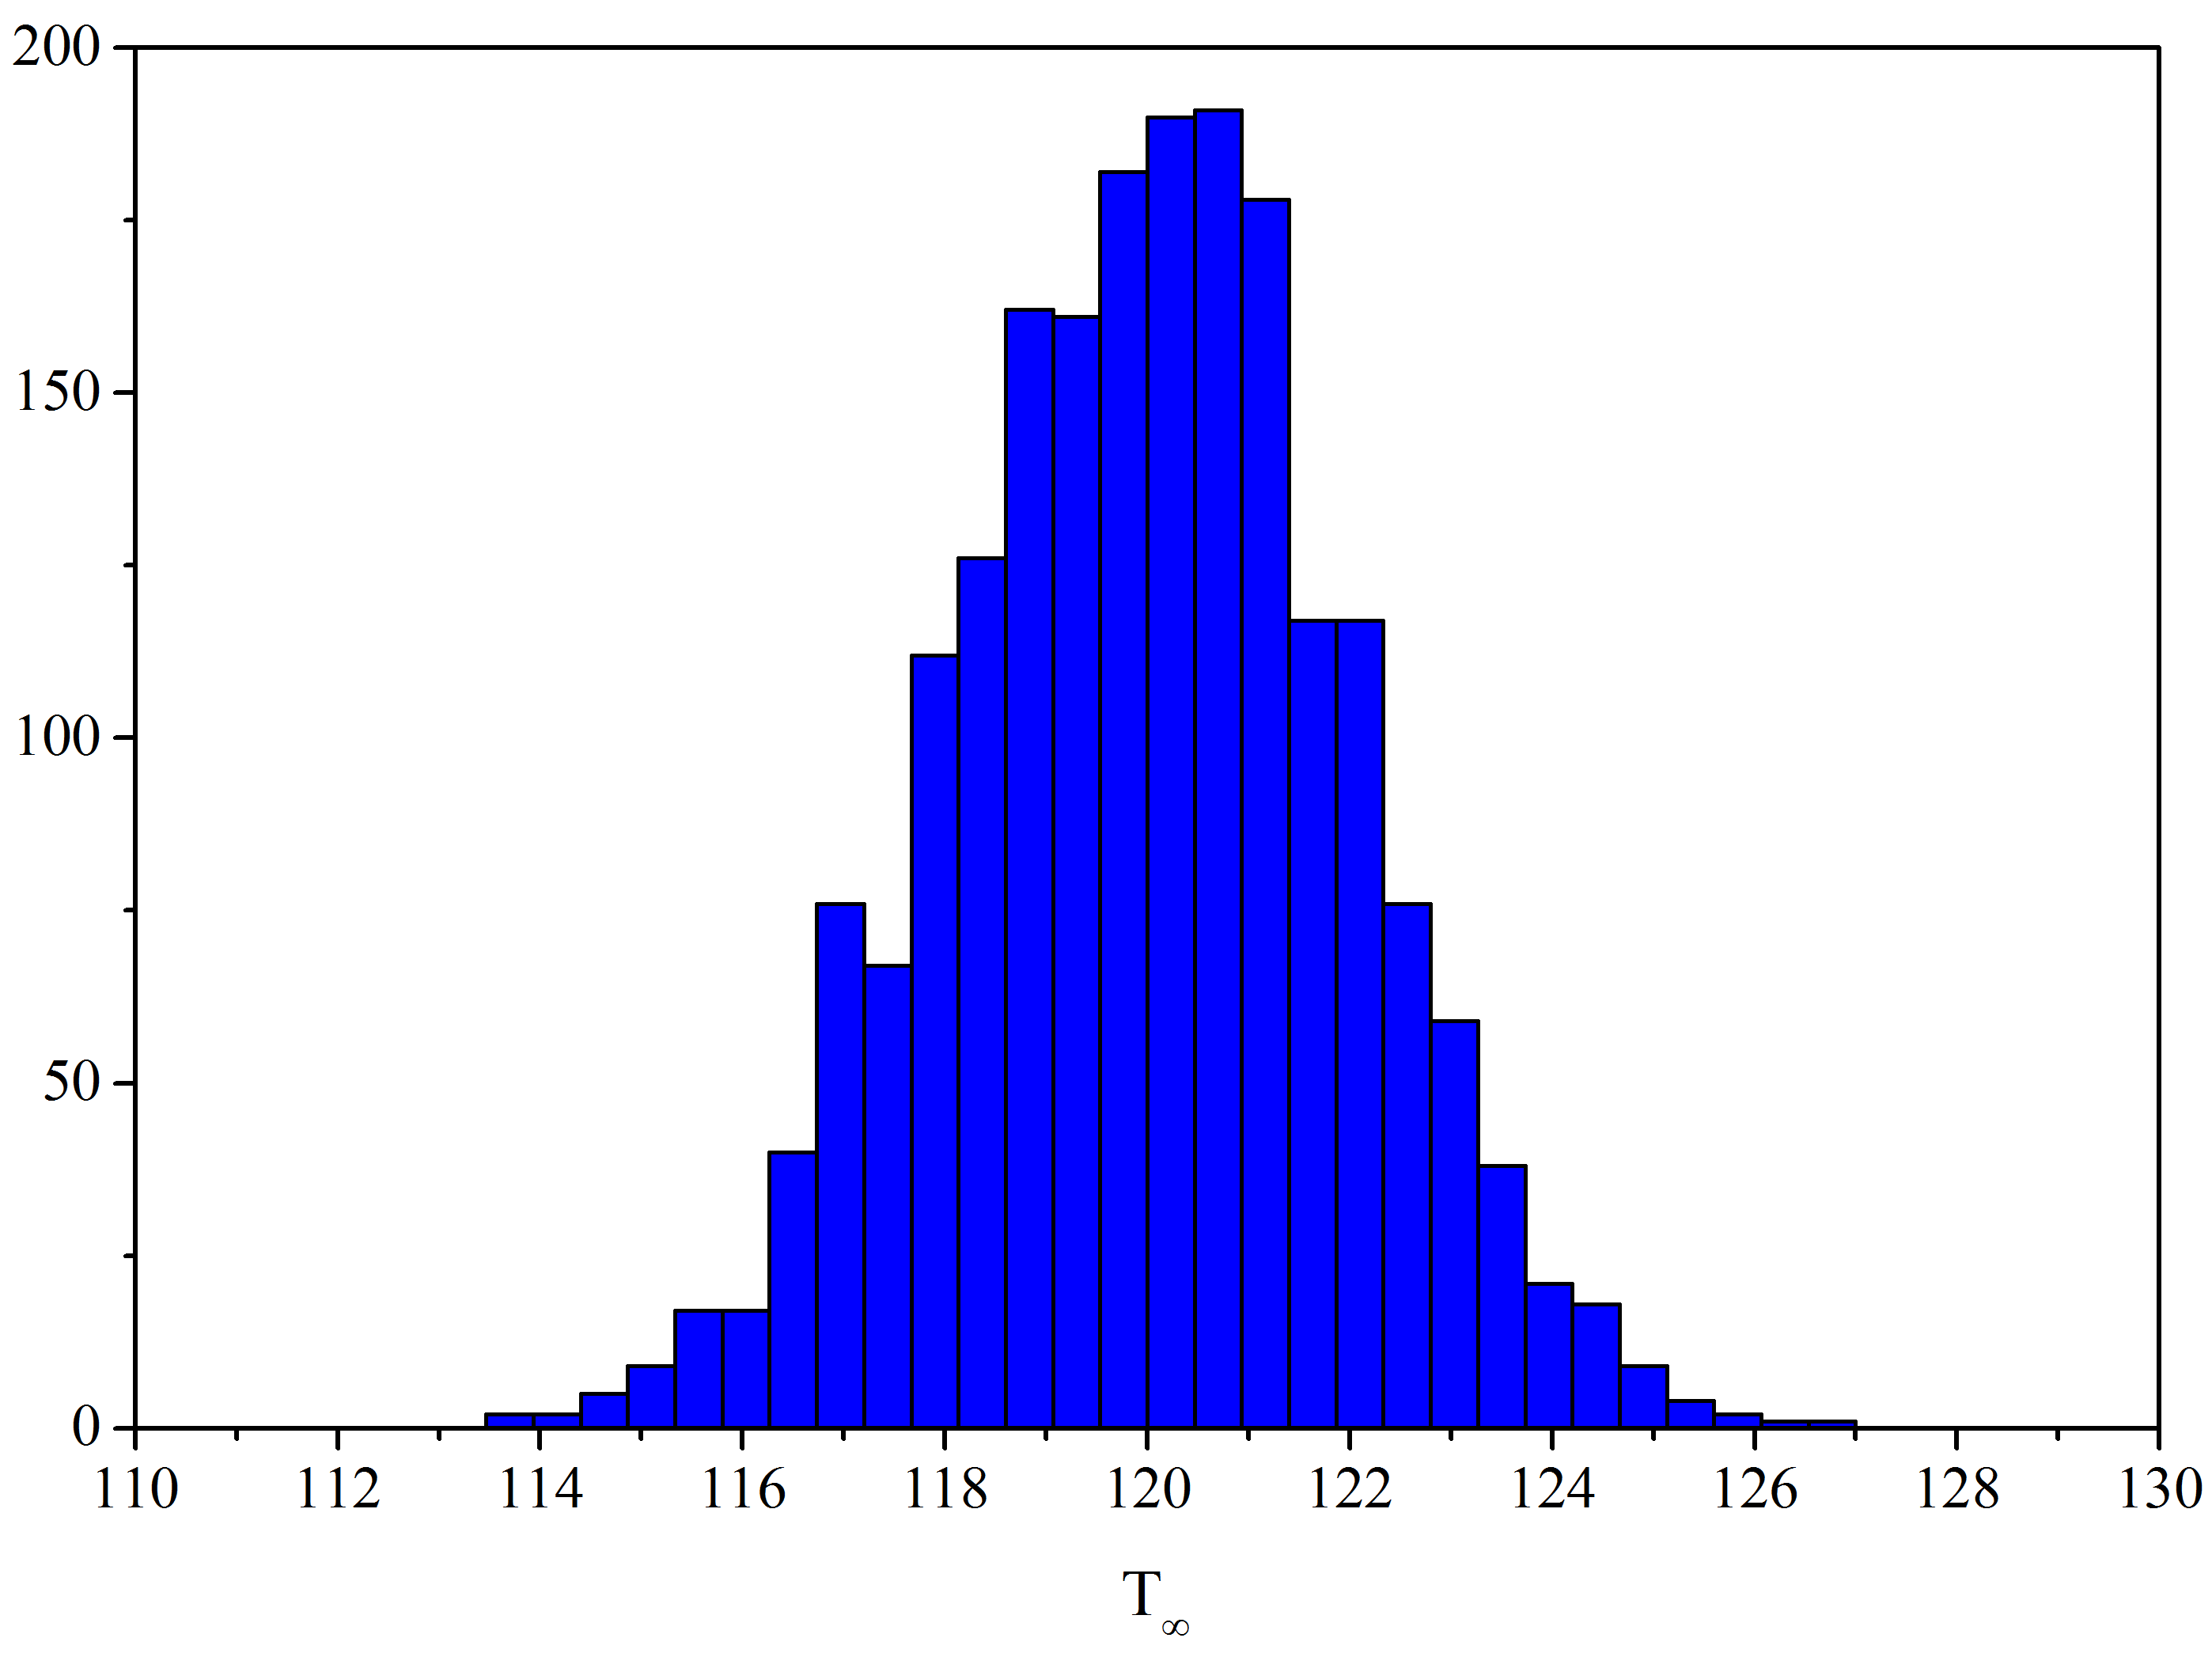
\includegraphics[width=0.45\textwidth]{./fig/Prior_right_T.png}}

\caption{The priors of unknowns of 3D heat sink}
\label{fig:prior_3D}
\end{figure}

\begin{figure}
\centering
\subfloat[The Robin boundary condition at left]{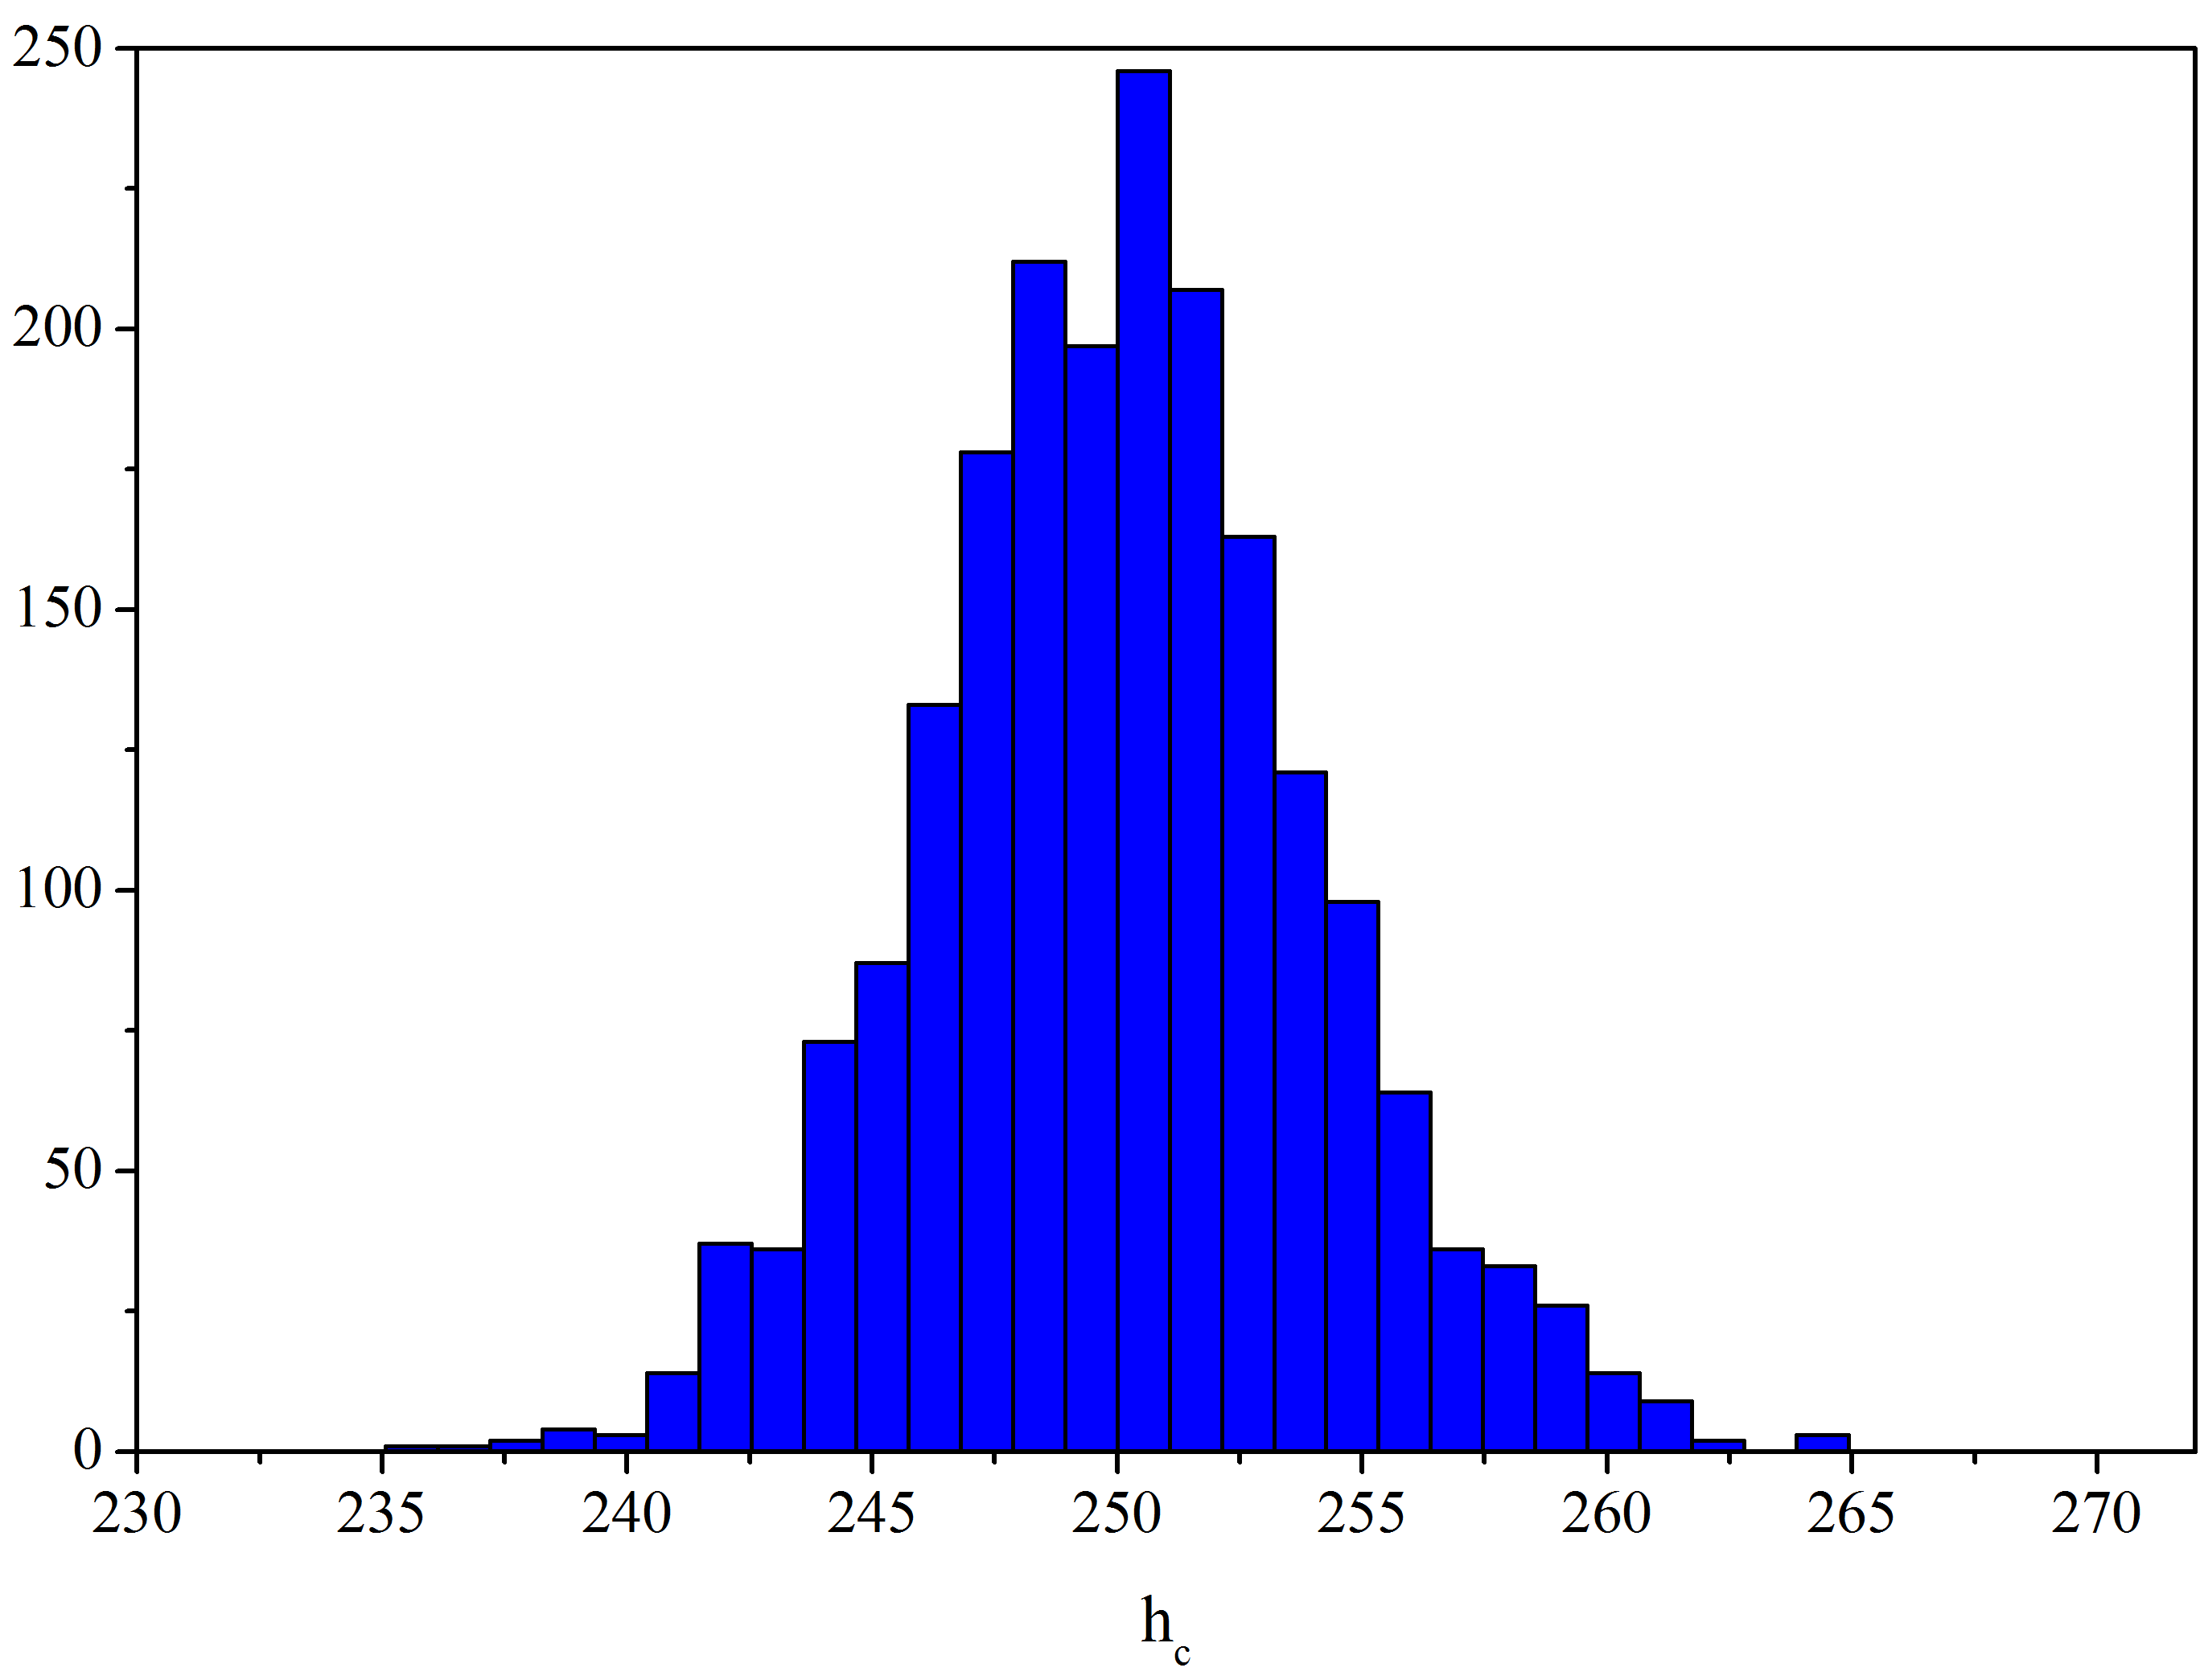
\includegraphics[width=0.45\textwidth]{./fig/Post_left_hc.png}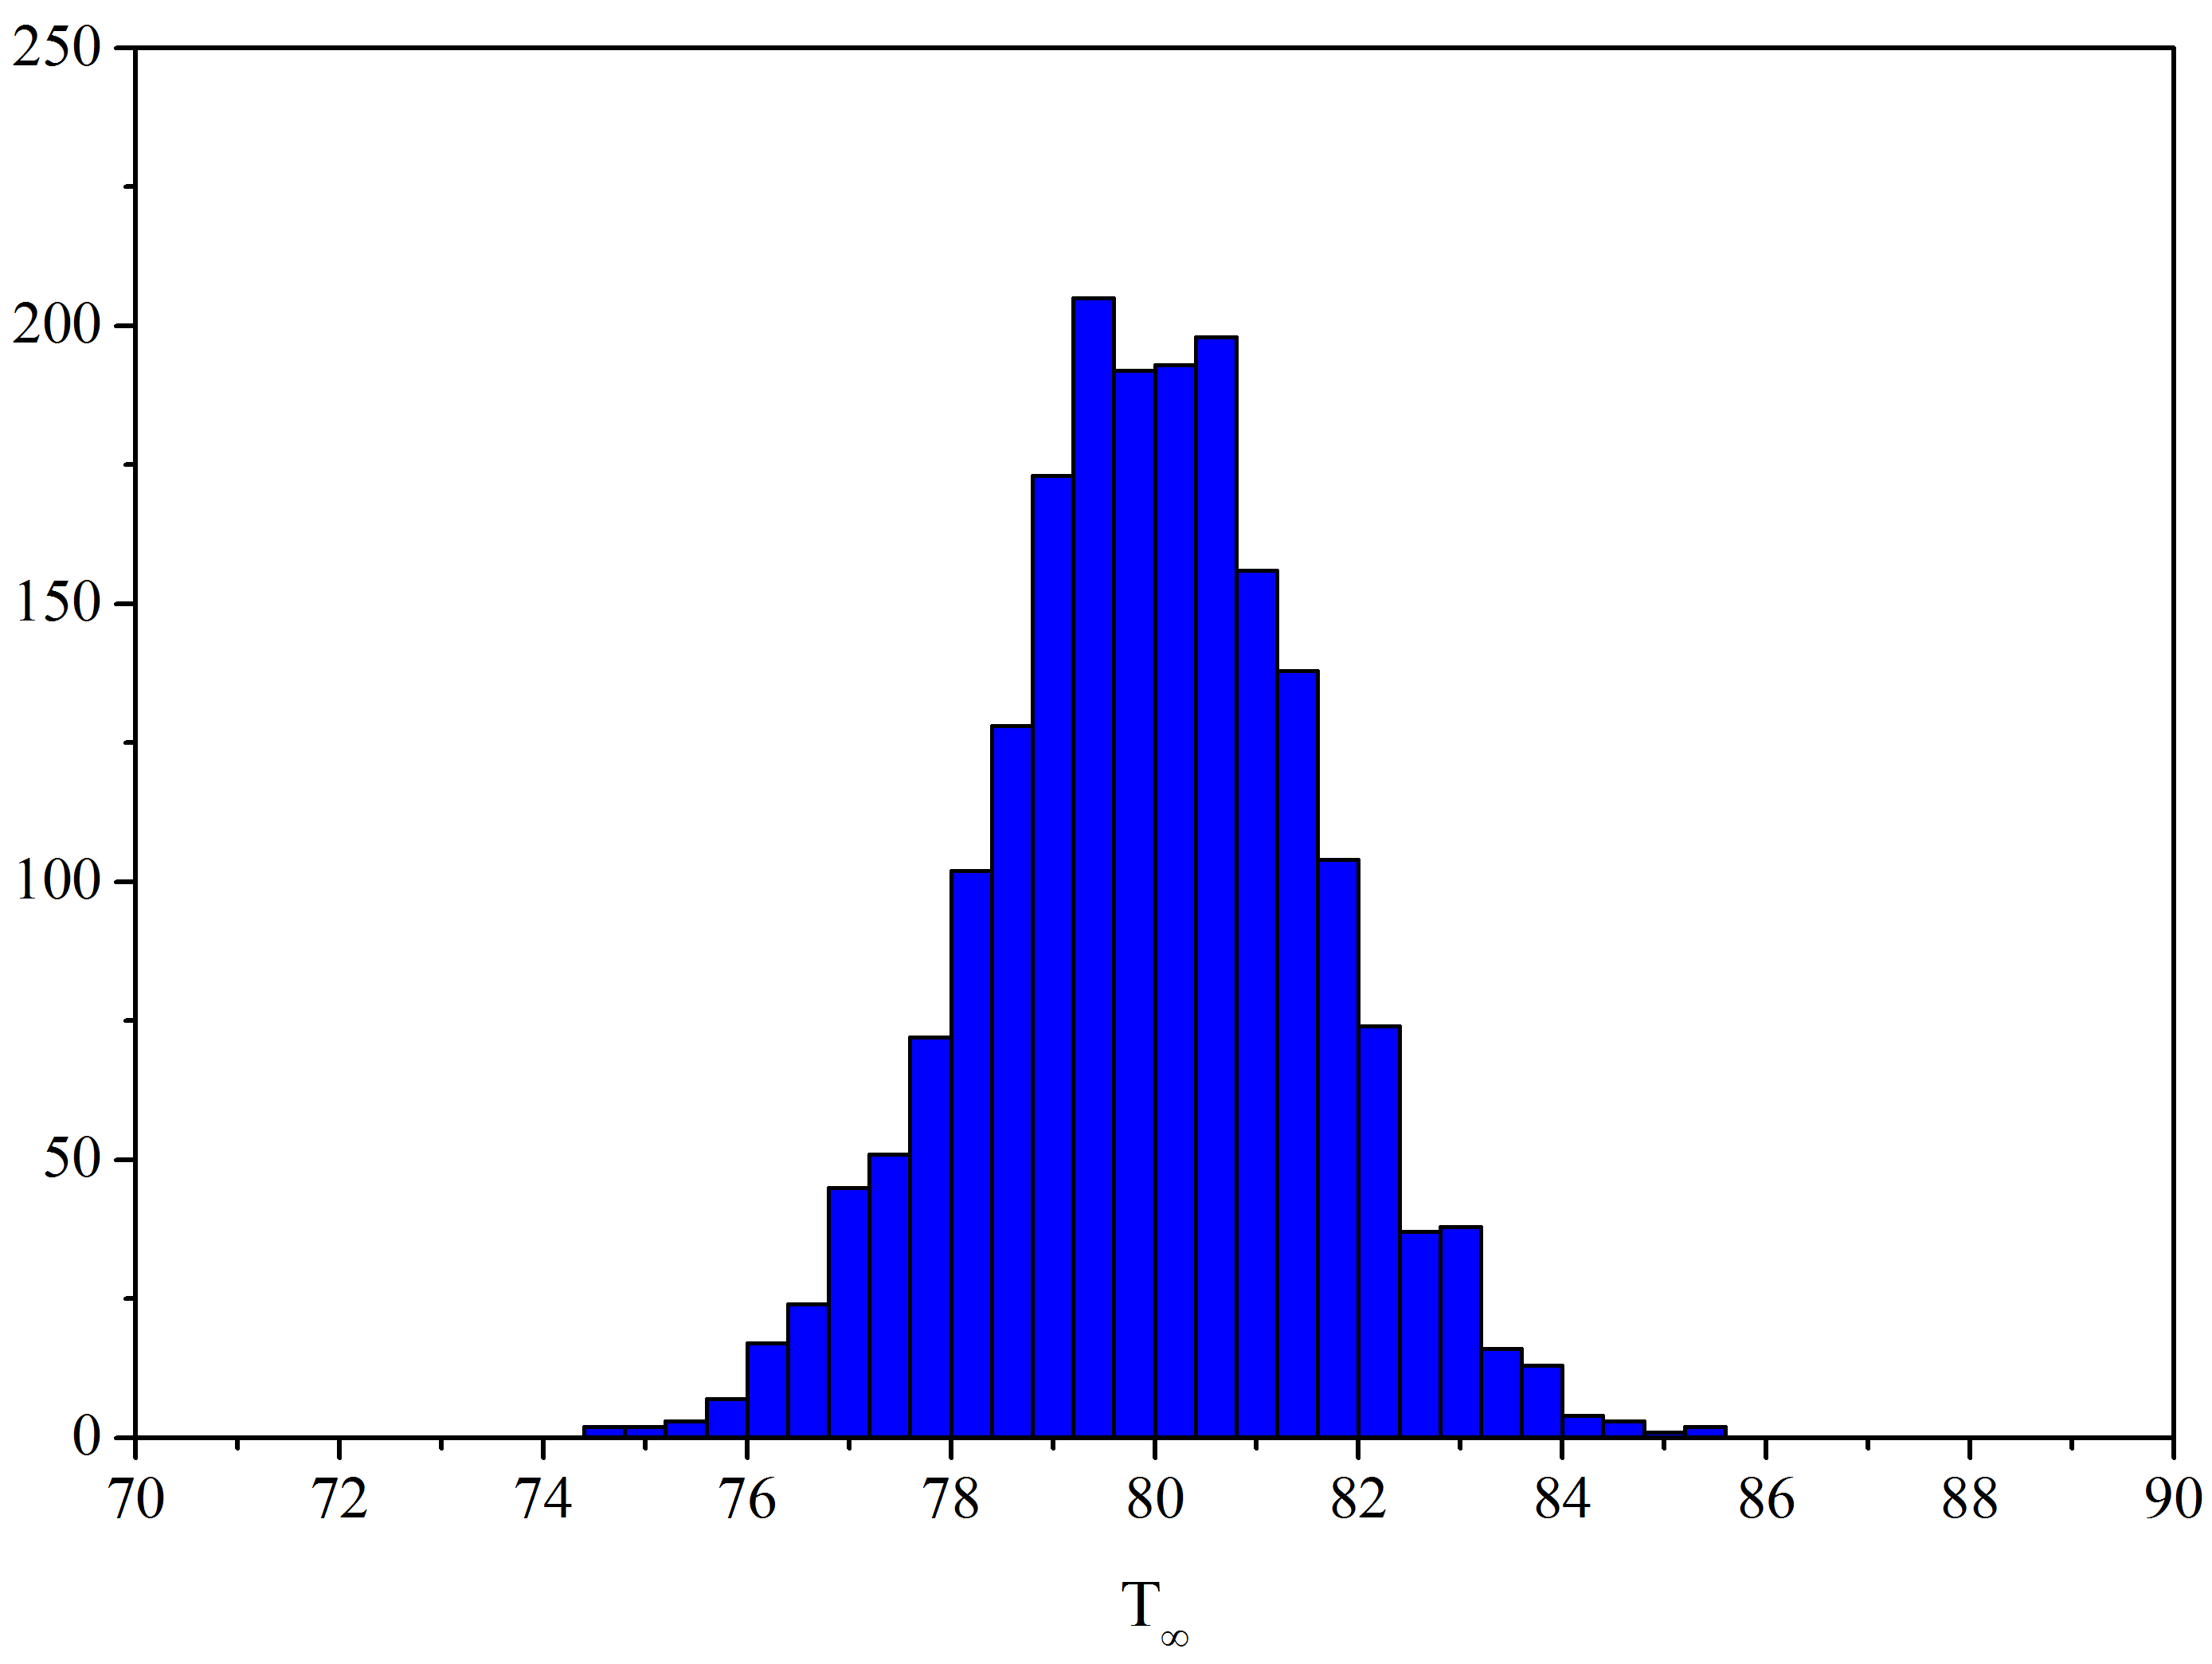
\includegraphics[width=0.45\textwidth]{./fig/Post_left_T.png}}

\subfloat[The Robin boundary condition at right]{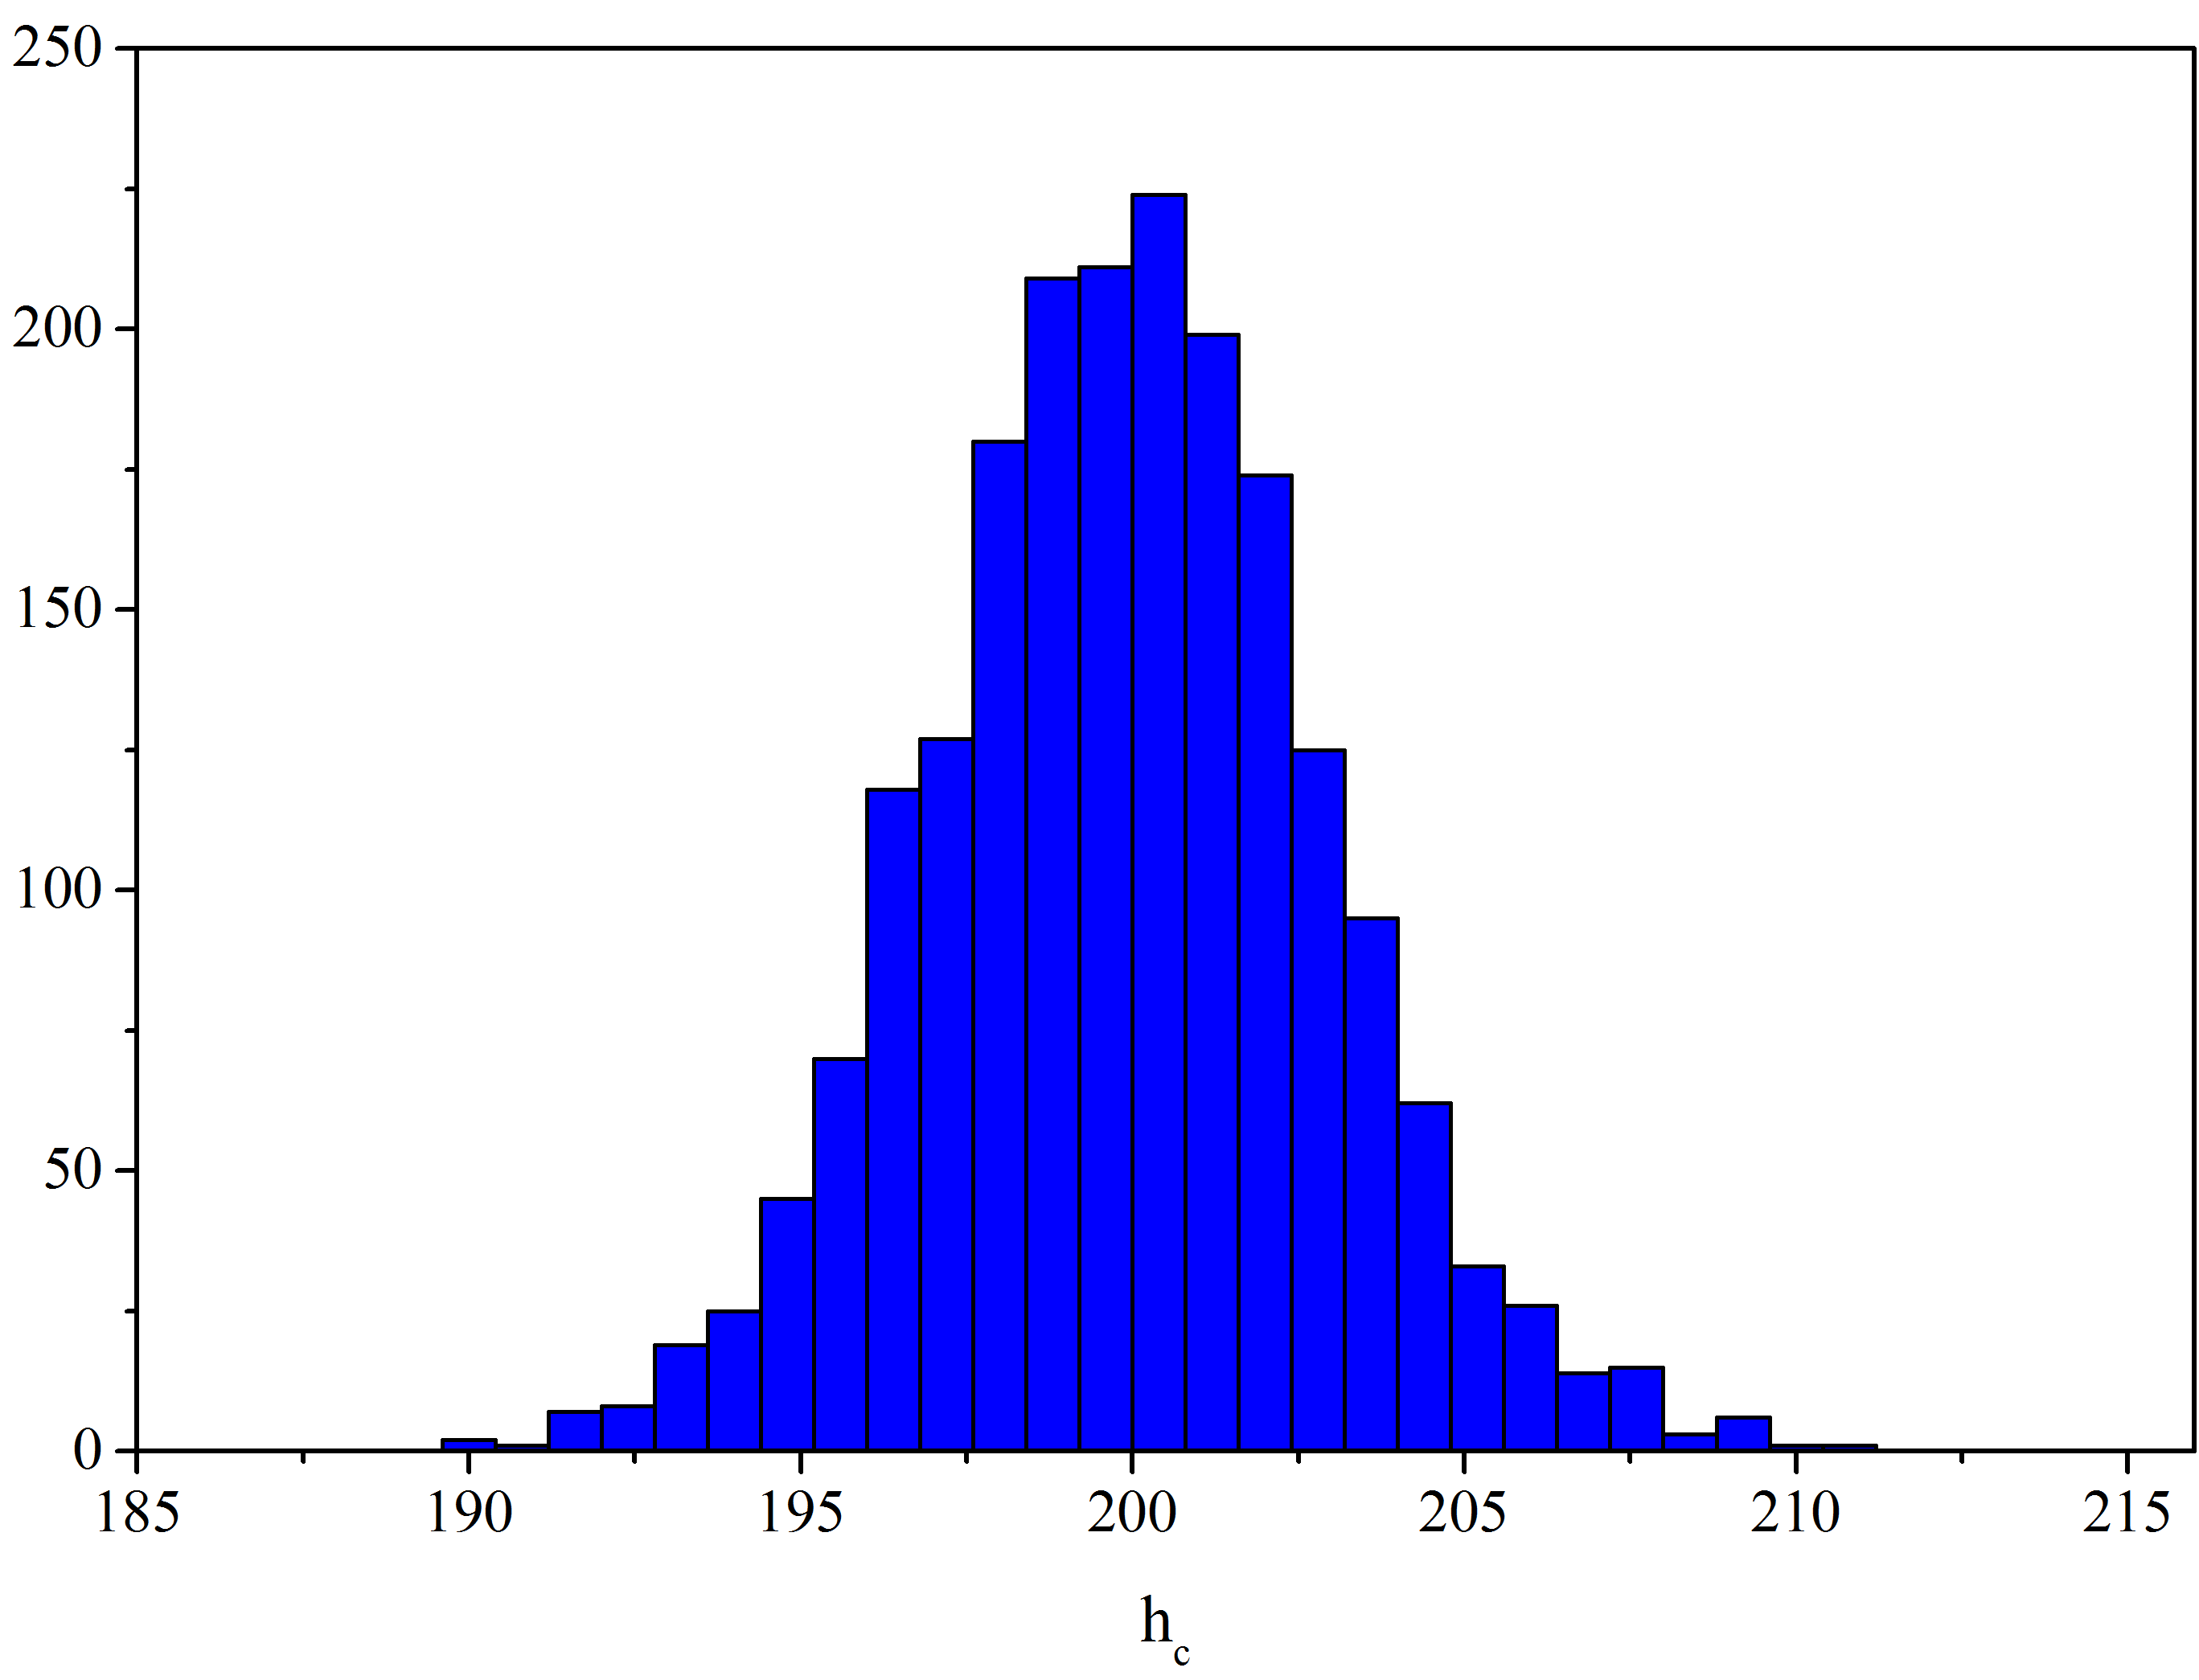
\includegraphics[width=0.45\textwidth]{./fig/Post_right_hc.png}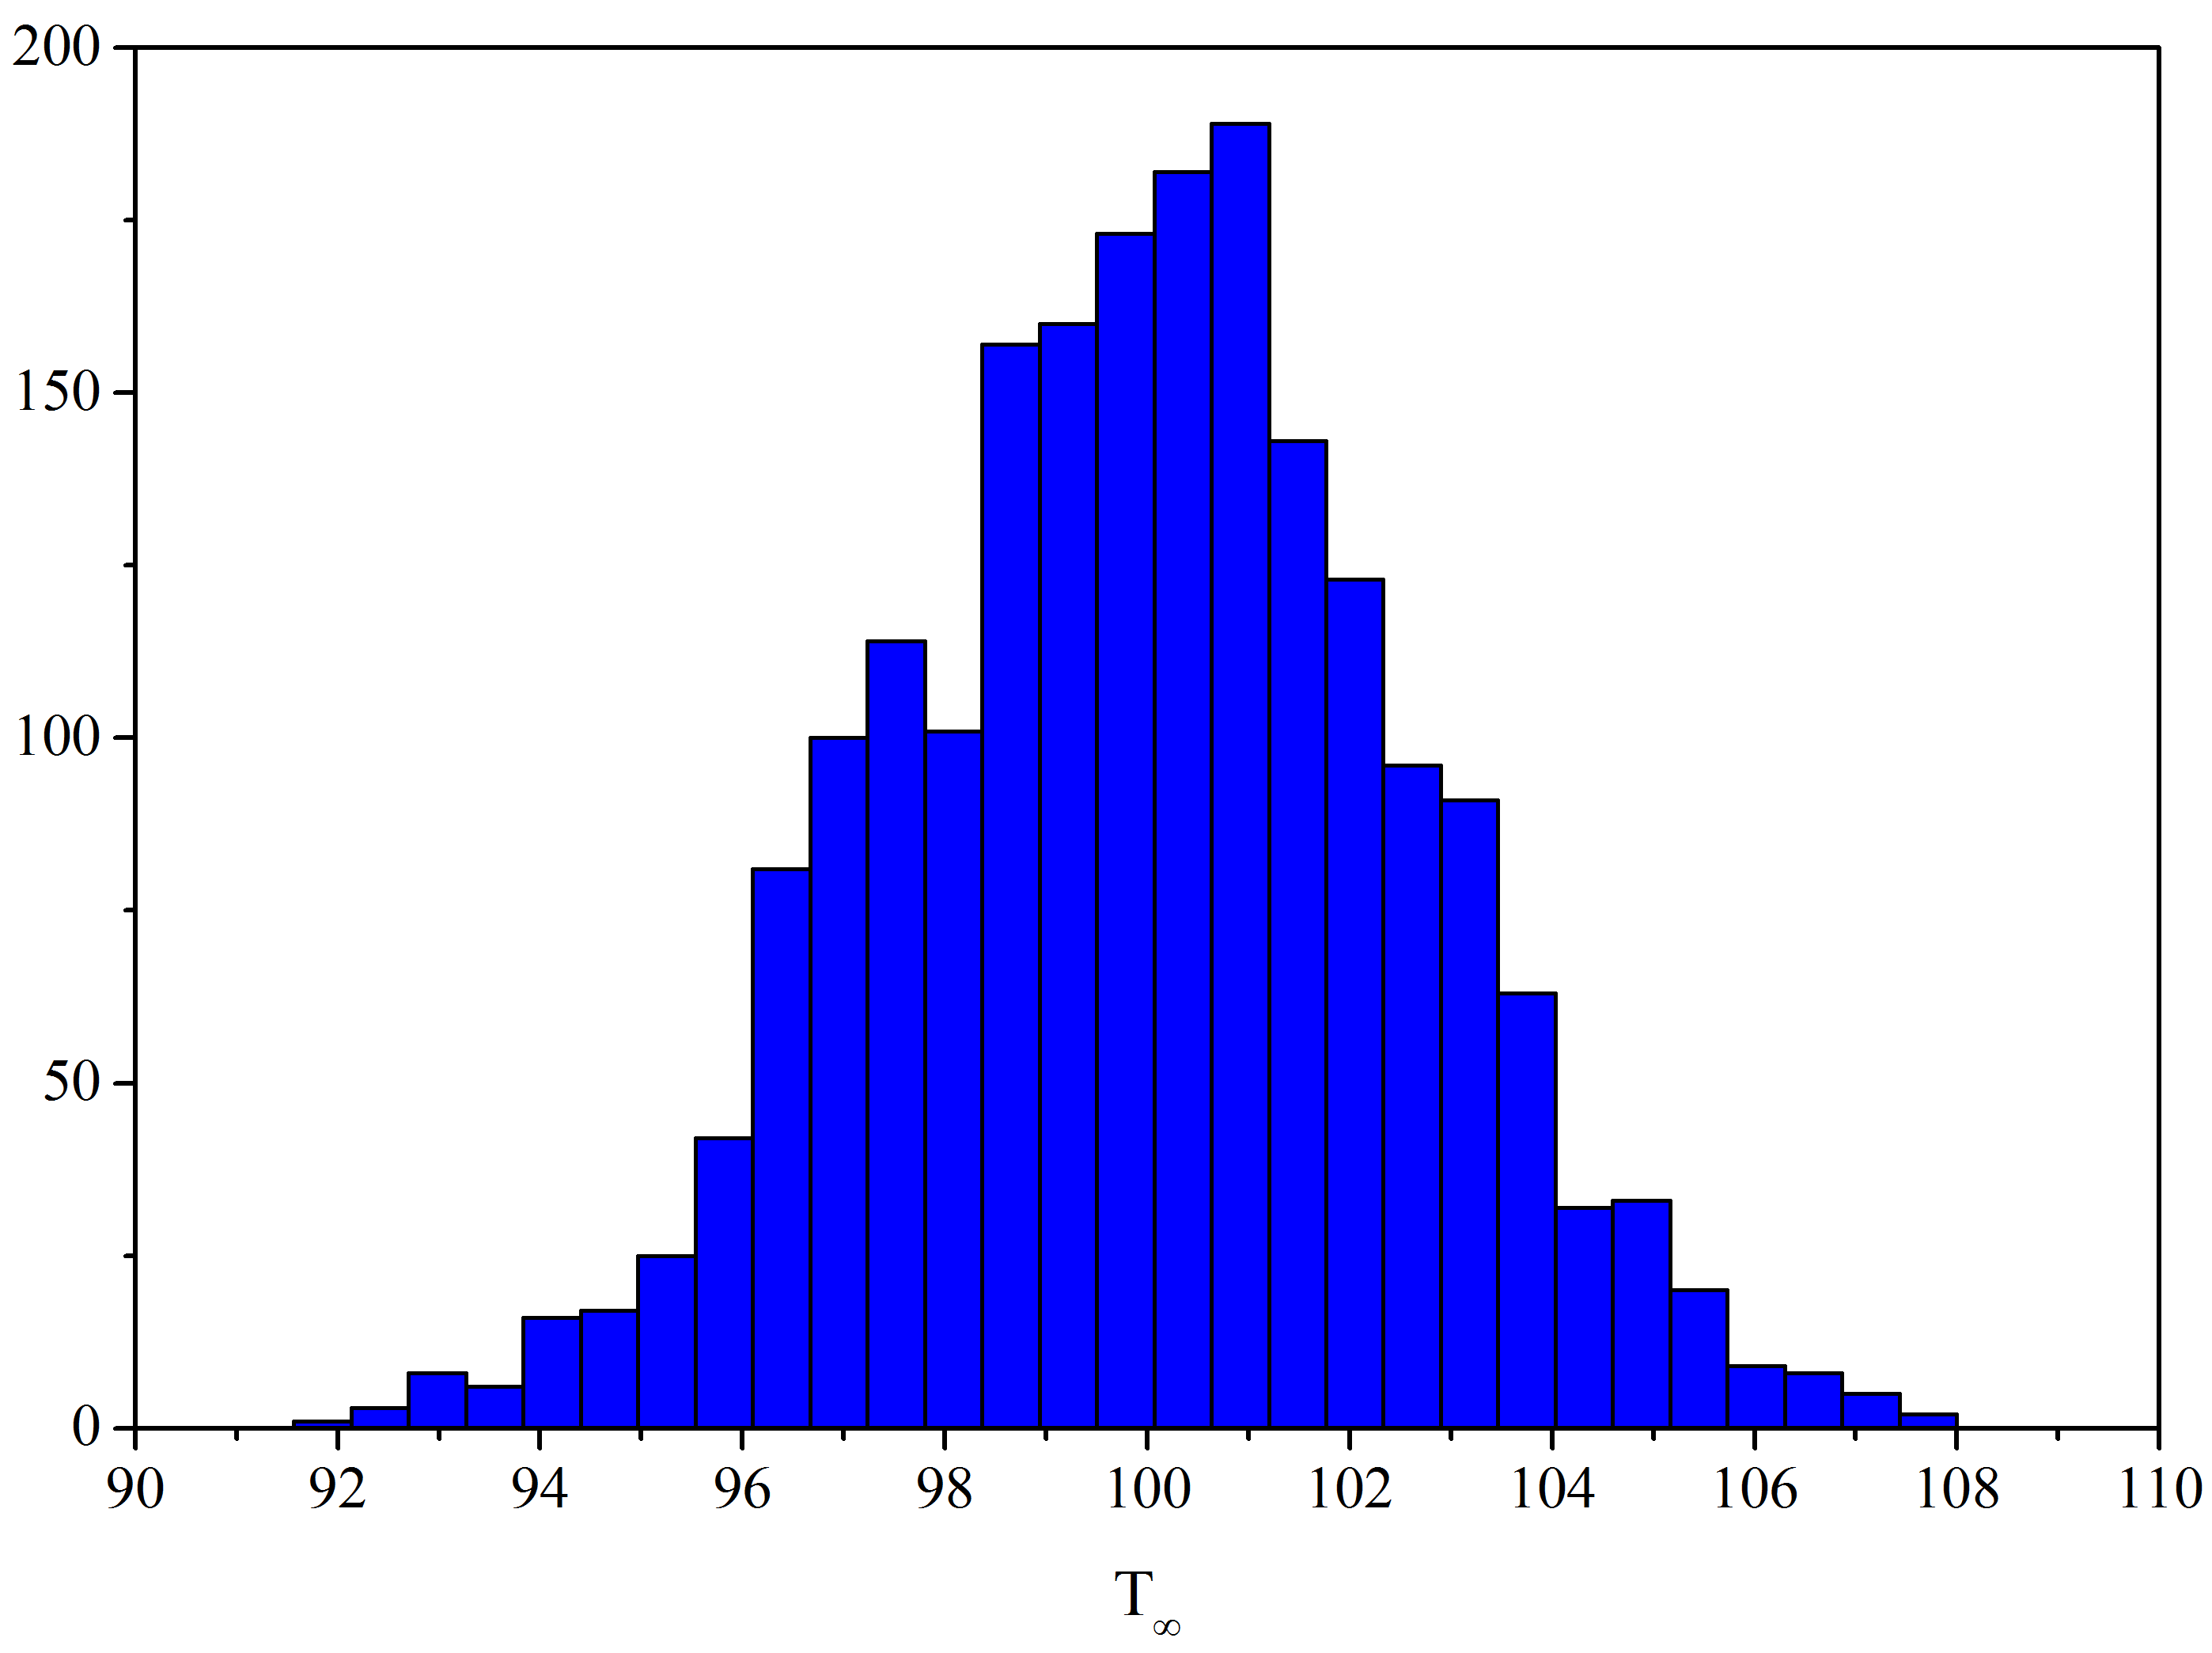
\includegraphics[width=0.45\textwidth]{./fig/Post_right_T.png}}

\caption{The posteriors of unknowns of 3D heat sink}
\label{fig:post_3D}
\end{figure}


\section{Conclusion}
In this study, an adaptive reanalysis based ABC-NPMC method are proposed to determine the unknown boundary conditions of static and nonlinear dynamic IHCP. In order to improve the convergence ratio of the ABC, the NPMC is was proposed. It firstly figures out the relationship between computational cost and tolerance value by predefined the sample pool. Then via optimization, it can obtain the more suitable tolerance value which can reduce computational cost significantly. Furthermore, in the entire process of the suggested method, no extra parameters are needed. It is also easily implemented. As validated by benchmark, it can reach a high efficiency.
Different fast computational methods are suggested for static and dynamical problems in which there are some modifications in the equilibrium equation such as the IHCP in this study. A superposition principle based solver is proposed for the static IHCP. It bypasses solving the inverse matrix of the FEM which is always time-consuming. As shown in the static example, it is much more efficient than the FEM with the same accuracy. As for the nonlinear dynamic IHCP, the CA reanalysis is extended to address the modifications of conduction matrix which is caused by the modified temperature field at each iteration. It addresses the modifications with a basis vector which is much smaller than the degree of freedom in conduction matrix. As proved in dynamic example, it is far more efficient compared with FEM with high accuracy.
With these examples, it can be shown that the estimations of the ABC are approaching the exact value with a proper tolerance threshold. Moreover, the ABC avoids the intractable likelihood function. Therefore, when tackling the practical engineering inverse problems, the ABC-NPMC would be a preferable alternative.
Generally, the main contributions of this study can be summarized as:
\begin{itemize}
    \item The ABC which can avoid the intractable likelihood function due to either computationally prohibitive or analytically unavailable is applied to the IHCP. 
    \item An adaptive NPMC is proposed. It can determine the tolerance value adaptively and need no extra parameters efficiently. 
    \item For static problem, superposition principle based heat conduction solver is utilized. As for dynamic problem, reanalysis based heat conduction solvers are developed to reduce the computational cost of simulations. Compared with FEM, it is far more efficient with a high accuracy.
\end{itemize}




\section*{Reference}

\bibliographystyle{elsarticle-num}
\bibliography{reference}

\section*{Appendix}

\begin{algorithm}
\caption{Preliminary Non-Parametric Population Monte Carlo method}
\label{al:1}
\begin{algorithmic}[1]
\STATE Input: Number of particles $N$, size of sample pool $N_p$, the stopping threshold $\varepsilon_s$
\FOR{$i=1:N_p$}
    \STATE Sample $\theta_i \sim P(\theta)$ and simulate $d(S(\theta),S(D))$,Sort $\theta_i$ with $d$.
    \STATE Calculate $\log{N_{need}}$ and determine the $\varepsilon_1$ with Eq.\ref{eq:Man}\ref{eq:Euc}\ref{eq:che}.
    \STATE Accept $\theta^{1_i} = \theta_i$ with $d < \varepsilon_1$
\ENDFOR
\FOR{$i = (N_a+1):N$}
    \STATE Simulate $\theta_i \sim P(\theta)$ and accept it with $d<\varepsilon_1$
\ENDFOR
\STATE Set $\Theta^{1} = [\theta^1_1,\theta^1_2,\cdots, \theta^1_N]$, $w^1_i = 1/N$ and $\sigma^1 = 2 var(\theta^1_{1:N})$
\WHILE{$\varepsilon_t>\varepsilon_s$}
    \STATE $t=t+1$, Sample $\theta^*$ from $\Theta^{t-1}$ with weight $w^1$, generate $\theta^{**} \sim q(\theta|\theta^*)$
    \STATE Sort $\theta^{**}_i$ with $d$, Determine $\varepsilon_t$ with Eq.\ref{eq:Man}\ref{eq:Euc}\ref{eq:che}.
    \STATE Accept $\theta^{**}_i$ with $d < \varepsilon_t$
    \STATE Sample and accept $N-N_\alpha$ $\theta^{**}_i$
    \STATE Set $w_t^t\propto P(\theta^{t}_i)/\sum_{j=1}^{N}q(\theta_t^i|\theta_j^{t-1})$ and $\sigma^t = 2 var(\theta^{t}_{1:N})$
\ENDWHILE
\end{algorithmic}
\end{algorithm}


\begin{algorithm}
\caption{Non-Parametric Population Monte Carlo method}
\label{al:2}
\begin{algorithmic}[1]
\STATE Input: Number of particles $N$, size of sample pool $N_p$, the stopping threshold $\varepsilon_s$
\FOR{$i=1:N_p$}
    \STATE Sample $\theta_i \sim P(\theta)$ and simulate $d(S(\theta),S(D))$,Sort $\theta_i$ with $d$.
    \STATE Calculate $\log{N_{need}}$ and determine the $\varepsilon_1$ with Eq.\ref{eq:Man}\ref{eq:Euc}\ref{eq:che}.
    \STATE Accept $\theta^{1_i} = \theta_i$ with $d < \varepsilon_1$
\ENDFOR
\FOR{$i = (N_a+1):N$}
    \STATE Simulate $\theta_i \sim P(\theta)$ and accept it with $d<\varepsilon_1$
\ENDFOR
\STATE Set $\Theta^{1} = [\theta^1_1,\theta^1_2,\cdots, \theta^1_N]$, $w^1_i = 1/N$ and $\sigma^1 = 2 var(\theta^1_{1:N})$
\WHILE{$\varepsilon_t>\varepsilon_s$}
    \STATE $t=t+1$, Sample $\theta^*$ from $\Theta^{t-1}$ with weight $w^1$, generate $\theta^{**} \sim q(\theta|\theta^*)$
    \STATE Sort $\theta^{**}_i$ with $d$, Determine $\varepsilon_t$ with Eq.\ref{eq:Man}\ref{eq:Euc}\ref{eq:che}.
    \STATE Accept $\theta^{**}_i$ with $d < \varepsilon_t$
    \STATE Accept $(N_{in})$ $\theta \in \Theta^{t-1}$ with $d < \varepsilon_t$
    \IF{$N-N_\alpha-N_{in} > 0$}
        \STATE Sample and accept $(N-N_\alpha-N_{in})$ $\theta^{**}_i$
    \ENDIF
    \STATE Set $w_t^t\propto P(\theta^{t}_i)/\sum_{j=1}^{N}q(\theta_t^i|\theta_j^{t-1})$ and $\sigma^t = 2 var(\theta^{t}_{1:N})$
\ENDWHILE
\end{algorithmic}
\end{algorithm}

\end{document}
